% \documentclass[sigconf, anonymous]{acmart}
\documentclass[sigconf]{acmart}

\usepackage{booktabs} % For formal tables
\usepackage{graphicx}
% Note: do not use url & hyperref packages.
% They do not pass the IEEE pdfxpress checks
% \usepackage{url}
% \usepackage{hyperref}
% \usepackage{subfigure}
\usepackage{balance}
\usepackage{amssymb,amsmath}
% \usepackage[usenames,dvipsnames,svgnames,table]{xcolor}
\usepackage{algorithm2e}
\usepackage{algpseudocode}

\usepackage{todonotes} % get rid of this later
\usepackage{subfig}
\usepackage{wrapfig}
\newcommand{\compactimg}{\vspace{-14pt}}
\newcommand{\tableref}[1]{Table~\ref{tab:#1}}
\newcommand{\figref}[1]{Figure~\ref{fig:#1}}
\newcommand{\secref}[1]{Section~\ref{sec:#1}}
\newcommand{\algoref}[1]{Algorithm~\ref{algo:#1}}

\newcommand{\bob}[1]{\textcolor{red}{{\bf from Bob: #1}}}
\newcommand{\cmt}[2]{{\color{blue} #1} {\color{red} [#2]}}

\newenvironment{tightitem}{\begin{itemize}\setlength{\itemsep}{1pt}\setlength{\parskip}{0pt}\setlength{\parsep}{0pt}}{\end{itemize}}

\begin{document}

% Copyright
\setcopyright{none}
%\setcopyright{acmcopyright}
%\setcopyright{acmlicensed}
% \setcopyright{rightsretained}
%\setcopyright{usgov}
%\setcopyright{usgovmixed}
%\setcopyright{cagov}
%\setcopyright{cagovmixed}


% DOI
\acmDOI{None}

% ISBN
\acmISBN{}

%Conference
\acmConference[IPSN]{IPSN}{2018}{Porto} 
\acmYear{2018}
\copyrightyear{2018}

\acmPrice{xx.00}

\title{ Charm: Exploiting Geographical Diversity Through \\ Coherent Combining in Low-Power Wide-Area Networks }

%\titlenote{Produces the permission block, and
%  copyright information}
% \subtitle{Extended Abstract}
% \subtitlenote{The full version of the author's guide is available as
%   \texttt{acmart.pdf} document}

\author{Adwait Dongare, Revathy Narayanan, Akshay Gadre, Anh Luong, Artur Balanuta, \\ Bob Iannucci, Swarun Kumar, Anthony Rowe }
\affiliation{%
 \institution{Carnegie Mellon University}
 \department{Electrical and Computer Engineering}
 % \streetaddress{5000 Forbes Ave.}
 \city{Pittsburgh, Pennsylvania} 
 % \state{Pennsylvania} 
 % \postcode{12345}
}
\email{ [adongare, revathyn, agadre, aluong2, arturb, roberti, swarunk, agr] @andrew.cmu.edu }

% The default list of authors is too long for headers}
\renewcommand{\shortauthors}{Dongare et al.}


\begin{abstract}


Low-Power Wide Area Networks (LP-WANs) are an emerging wireless platform which
can support battery-powered devices lasting 10-years, while communicating at
low data-rates to gateways several miles away. Yet, despite the expected
high-density of LP-WAN gateways in future cities, not all devices will
experience the promised 10-year battery life, particularly in urban spaces. A
large number of devices that are deep inside buildings, or in remote
neighborhoods would suffer severe battery-drain due to extended transmissions
at the slowest data rate to reach even the closest gateway.

This paper presents Charm, a system that enhances both battery life and
coverage of LP-WAN clients in large urban deployments. Charm allows multiple
LoRaWAN gateways to pool their received signals in the cloud, coherently
combining them to detect even the weakest signal that is not decodable at any
individual gateway. Charm achieves this through a novel hardware and software
design at the gateway that carefully detects which chunks of the received
signal need to be sent to the cloud, thereby saving uplink bandwidth. We
demonstrate how our solution scales to decoding weak transmissions at
city-scale, by identifying the set of gateways whose signals need to be
coherently combined over time. In evaluations over a test network and from
simulations using traces from a large LoRaWAN deployment in Pittsburgh, Charm
demonstrates a significant gain of 3$\times$ in range and 4$\times$ in client
battery-life.

\end{abstract}

%used to add page numbers
\settopmatter{printfolios=true}

\maketitle


\section{Introduction}
\label{sec:intro}

Low Power Wide Area Networks (LPWANs) are increasingly seen as an attractive
communication platform for city-scale Internet-of-Things (IoT) deployments.
They offer the ability to wirelessly connect energy-constrained devices to
gateways over distances of many kilometers. LPWANs also have power and cost
advantages over alternatives like cellular networks, particularly in
deploy-once, low maintenance and low throughput sensing applications.

While LPWANs are far from pervasive, the capabilities of networks like
LoRaWAN~\cite{Sornin2015, LoRaWanAlliance2015}, SigFox~\cite{centenaro2016}
and Ingenu's RPMA~\cite{Ingenu2015} have attracted investment and have spawned
early deployments. These technologies operate on the unlicensed ISM spectrum,
allowing businesses and consumers alike to deploy their own devices and
gateways. With Comcast recently announcing integration of LPWAN radios into
future set-top boxes in the U.S.~\cite{comcast2}, LPWANs are likely
to grow rapidly. Given that each LPWAN gateway promises a range of up to ten
kilometers~\cite{LoRaWanAlliance2015}, major cities are likely to see a
fast-paced expansion in LPWAN coverage.

Despite the expected rise in density of LPWAN gateways, not all devices will
experience the promised 10 year battery life. Devices located in urban spaces
deep inside buildings or in remote neighborhoods will experience severe drain
in battery as their signals are highly attenuated even at the closest base
station. Some of these devices, such as those in basements or tunnels, may not
be in communication range of any gateway at all. Unlike cellular networks,
LPWANs are largely user-deployed and unplanned, meaning that these devices may
remain battery deprived or simply out of network reach in perpetuity, even as
thousands of gateways proliferate city-wide.

\begin{figure}[tb]
    \centering
    % \vspace{-10pt}
    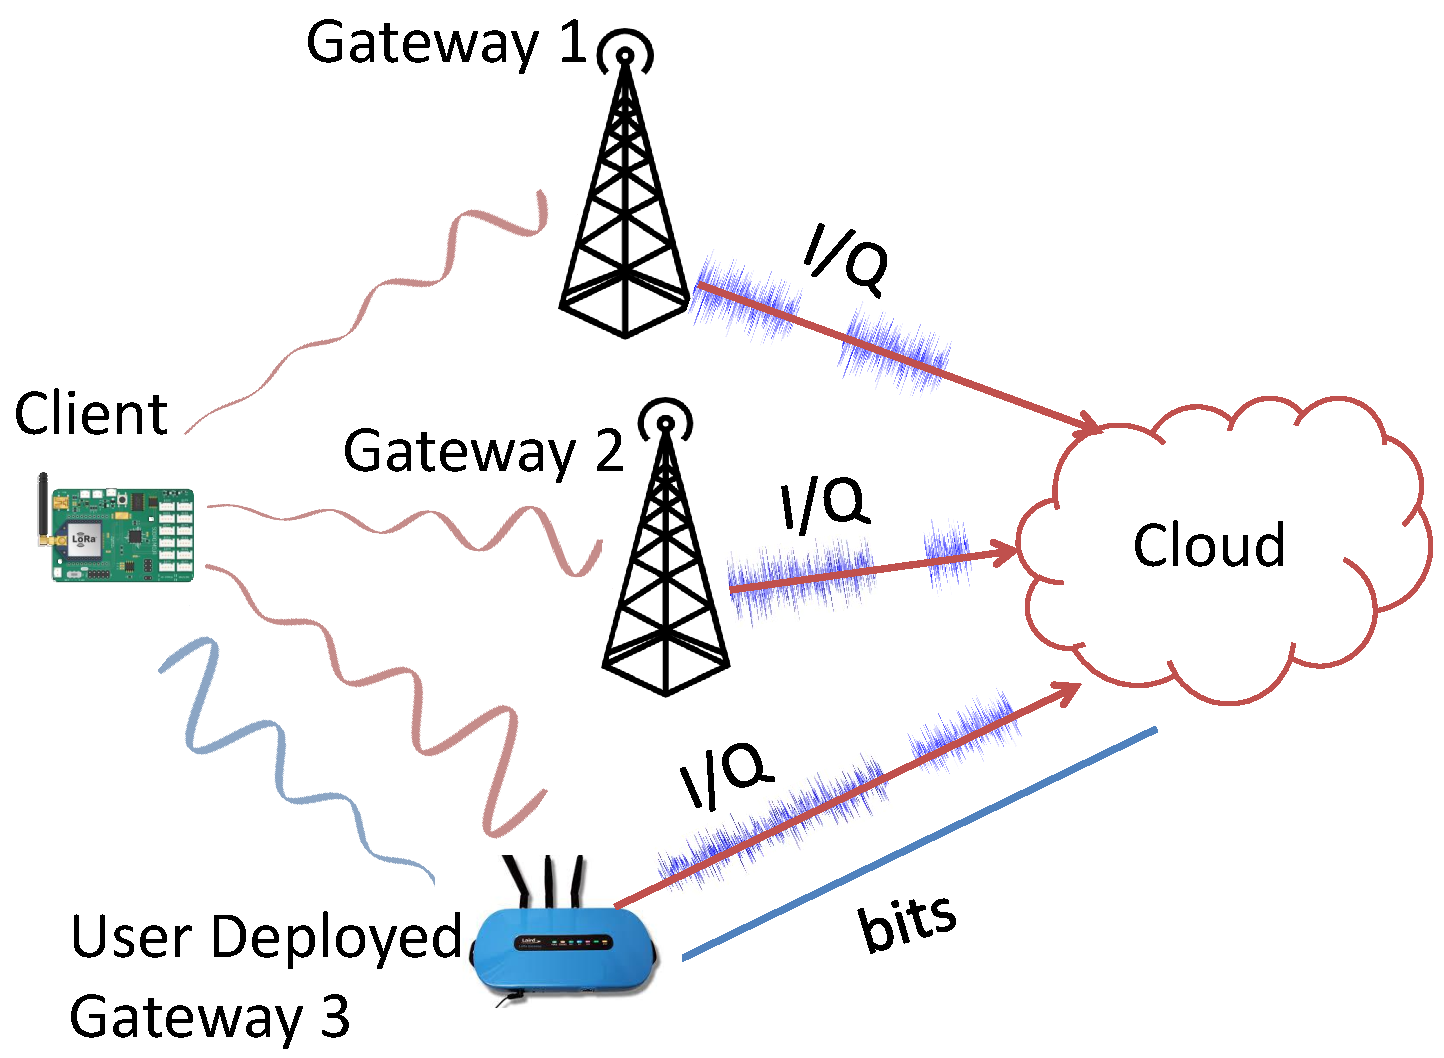
\includegraphics[width=0.60\columnwidth]{figures/LoRaRAN_cropped}
    \vspace*{-10 pt}
    \caption{Charm: LPWAN joint decoding in the cloud}
    \compactimg
    \label{fig:my_label}
\end{figure}

This paper presents Charm, a system that enhances the coverage of LPWANs and
the battery life of client devices in large urban deployments. Charm exploits
the observation that while signals from certain clients may attenuate
significantly, they are still likely to be received by multiple gateways in a
dense network. Charm introduces a hardware and software design at the gateways
that identifies and transports weak received signals to the cloud. We then
develop a joint decoding system at the cloud that coherently combines weak
signals received across multiple city gateways to decode the underlying data.
As a result, Charm both expands the decoding range of the LPWAN network and
improves battery-life for nodes already in range -- allowing client devices to
spend less energy per transmitted bit. Charm is built on the LoRaWAN
platform~\cite{LoRaWanAlliance2015}, a popular and widely available LPWAN
technology. Charm is implemented in a first-of-its-kind pilot deployment for
coherent diversity combining and demonstrates increased network coverage and
improved data rates across client devices.

While coherent diversity combining and PHY-layer processing in the cloud has
received much attention in the Wi-Fi~\cite{tan2009sam, xie2014scalable} and
cellular~\cite{checko2015cloud, wubben2014benefits} context, designing such a
system for low-power WANs offers radically new challenges. At the gateways, we
would have to decode very weak signals, weaker than 30 dB below the noise
floor. Simply uploading all received data to the cloud would overwhelm
the backend link, which is often  a simple home LAN. Both the LPWAN gateways
and clients are designed to be economical and deployed at scale, and without
the time synchronization required for coherent combining. At the cloud,
collating receptions from a large number of gateways at city-scale to identify
which of them contain packets from the same client is a challenge. We provide
an overview of our approach to address each of these challenges.

\noindent \textbf{Noise-Resilience at the Gateway:} The key challenge at the
gateway is identifying packets that are significantly below the noise floor
and, therefore, virtually undetectable. A straw-man approach to this problem
would be to correlate the received signal with a known preamble in any valid
packet. For instance, LoRaWAN uses a sequence of identical chirps -- signals
whose frequency increases linearly in time -- as a signature that is prefixed
in every packet. In principle, sending an extremely long preamble could
provide high resilience to noise. In practice, doing so goes against the
spirit of LPWANs where energy for transmission is a valuable resource for the
client.

Charm's approach to resolving this challenge is a hardware and software gateway
design that leverages the structure of the LoRaWAN LPWAN protocol.
Specifically, we develop a transform that converts the data symbols containing
\textit{a priori} unknown bits into a repeated and known sequence of signals,
much like the preamble. Charm can therefore now use both the preamble and the
modified data sequence to detect any packet.

To understand our approach at a high-level, we present an illustrative example
that dives into the details of the LoRaWAN PHY-layer. LoRaWAN transmits data
symbols as chirps whose initial frequency is a function of the data. For
instance over a bandwidth of 100 Hz, LoRa could represent the bit "0" as a
chirp starting at 2 Hz and bit "1" as a chirp starting at 52 Hz. Charm's
filter aliases the received LoRa signal so that frequencies modulo 50 Hz fold
into each other. This means that both bit "0" and bit "1" now map to an
identical chirp starting at 2 Hz. We apply this filter through the received
packet to obtain a repeated sequence of chirps as long as the entire packet
itself. This technique allows us to detect the packet with a much higher
resilience to noise compared to using the preamble alone, without incurring
additional overhead.

We develop a custom gateway hardware platform integrating a Semtech LoRaWAN
radio frontend, a low-power FPGA and Raspberry PI that can filter and detect
weak signals by processing received raw I/Q samples in real-time. Our hardware
platform, a hybrid between a full SDR and a dedicated high-performance radio,
is designed to be open and highly programmable -- a novel tool to experiment
with alternative LPWAN PHY-layer designs in the 900 MHz ISM band, without
compromising on signal quality or real-time performance.

\noindent \textbf{Scalability at the Cloud:} At the cloud, Charm must deal
with a large number of receptions from various gateways in a city, pruning for
weak signals and identifying common signals between gateways. Charm proposes
multiple optimizations to run its algorithms seamlessly at city-scale. For
instance, it is often the case that gateways transmit weak signals to the
cloud for packets that have already been decoded perfectly at other gateways.
However, realizing that the weak signal has already been decoded elsewhere is
impossible without decoding it in the cloud in the first place. Charm resolves
this chicken-or-egg dilemma by exploiting the timing and geographical location
of the received signal. Prior to sending any signal data to the cloud, a Charm
gateway sends the location, frequency, accurate timing and signal-to-noise
ratio (SNR) of the received weak packet. The cloud collates such information
across multiple gateways and requests for signals only from the gateways that
receive these signals the best. In doing so, Charm saves valuable uplink
bandwidth at the gateways and compution at the cloud. We describe how Charm
mitigates range of other important challenges at the cloud such as imperfect
timing, frequency offsets and overlapping transmissions.

We evaluate Charm in both indoor and outdoor environments using two testbeds
on the Carnegie Mellon University campus and around the city of Pittsburgh.
Eight user-deployed gateways built using our custom hardware platform support
a testbed covering a 0.6 sq.km. area around campus, which is used to study
Charm's performance with regard to local packet detection, range and
data-rates. Four rooftop gateways support the OpenChirp LPWAN network which
services a large 10 sq.km. area that we use to acquire traces for large-scale
simulations. Our results reveal the following:

\begin{itemize}
    \item {\bf Battery-Life: } By coherently combining across 8 base stations,
        Charm improves the SNR of a typical LoRaWAN transmission by 3.16 dB,
        extending battery life by up to 4$\times$.
    \item {\bf Range: } We improve the maximum communication range of 8 indoor
        user-deployed gateways in urban settings from 60m in LoRaWAN to 200
        meters using Charm, an overall increase in coverage area by
        10$\times$.
    \item {\bf Coverage: } Our trace-driven simulation, based on city-wide
        drive tests, estimates an overall increase in coverage area by up to 2x due
        to Charm over LoRaWAN.
\end{itemize}

\noindent \textbf{Contributions:} We make the following novel contributions:
\begin{itemize}
    \item A technique that leverages the geographical diversity of unplanned,
        user-deployed gateways to enable joint decoding of weak transmissions.
        This improves battery-life for users in the network and increases the
        coverage area.
    \item A hardware platform and the underlying algorithms for detecting weak
        LoRaWAN transmissions locally at the gateway.
    \item A software architecture that builds atop of LoRaWAN to enable
        joint-decoding of signals in a scalable manner.
\end{itemize}
\section{Related Work}
\label{sec:related-work}

% {\color{blue}
% [ANYTHONY, SWARUN, BOB, ARTUR, ADWAIT, DIANA, MAX]

% Particular topics to consider
% \begin{itemize}
% \item PerCom workshop paper
% \item Localization (Reverse GPS)
% \item WiFi and Cellular existing work
% \end{itemize}
% }

\noindent \textbf{Low-Power Wide-Area Networks: } Recent years have seen much
interest in Low-Power wide area networks (LP-WANs), including the development
of new hardware and standards. Private enterprises such as
Semtech~\cite{LoRaWanAlliance2015} and
SigFox~\cite{sanchez2016state} have developed LP-WAN chipsets that use extremely
narrow bands of unlicensed spectrum. In contrast, cellular standardization
bodies have developed two standards for LP-WAN communication for cellular base
stations to communicate with low-power IoT devices over licensed spectrum:
LTE-M~\cite{GSMAssociation2016} 
and NB-IOT~\cite{ratasuk2016nb}. 
Unlike LoRa and
SigFox, these technologies require devices to periodically wake up to
synchronize with the network -- a burden on battery life.

Several recent measurement studies have been conducted to evaluate the
performance and range of LP-WAN networks~\cite{petric2016measurements, toldov2016performance} and perform theoretical capacity
analysis~\cite{mikhaylov2016analysis}. Early pilot deployment efforts are also
underway with SigFox deploying their hardware to connect security alarms to
the cloud in Spain~\cite{sanchez2016state}, smart blood refrigerators in the
Democratic Republic of the Congo~\cite{ramachandranmupnp} and smart city
applications \cite{centenaro2015long}. These efforts motivate the challenge of
limited range, performance and battery-drain of LP-WAN clients. A recent system, Choir~\cite{eletreby2017empowering} has demonstrated improving range and scalability of LP-WANs through collaborations of weak client radios. In contrast, this paper seeks to use collaboration between gateways without any modifications to client behavior whatsoever to improve the battery life of even a single client. \\\vspace*{-0.1in}

\noindent \textbf{Distributed MIMO and Coherent Combining: } A large body of work has proposed the use of multiple-antennas (MIMO) to improve SNR and reduce interference~\cite{xie2014scalable, lin2011random, kumar2013bringing}. In the Wi-Fi context, past systems have used multi-user MIMO to improve performance on the uplink~\cite{shen2014rate, tan2009sam, xie2014scalable}. In the cellular context, massive MIMO proposals have demonstrated scaling gains of towers with a large number of antennas~\cite{shepard2012argos, larsson2014massive}. There has been much theoretical work on distributed MIMO overall in both the sensor networking context~\cite{del2007cooperative} and wireless LANs~\cite{dohler2004resource} and cellular networks~\cite{sawahashi2010coordinated}.  More recently, practical distributed MIMO systems, primarily in the LAN-context have demonstrated both multiplexing and diversity gains~\cite{hamed2016real, yenamandra2014vidyut, rahul2012jmb}. Instead, our approach brings the diversity gains of distributed MIMO on the uplink to low-power wide-area networks. In doing so, we overcome multiple challenges owing to the fact that signals at any individual tower are well below the noise floor. \\\vspace*{-0.1in}


\noindent \textbf{Cloud Radio Access Networks (Cloud-RAN): } Multiple research efforts from the industry and academia have advocated the use of PHY layer processing at the cloud as opposed to the base stations~\cite{sabella2013ran, hadzialic2013cloud}. In the cellular context, CloudRAN aims to perform baseband processing at the cloud, allowing base stations to be simple and easy to deploy~\cite{checko2015cloud, wubben2014benefits}. The key challenge however is the need for a reliable fiber optic backhaul to the cloud to collate data streams in a low latency manner, motivating the need for cost-effective high-performance backhauls~\cite{liu2013case, chih2014recent}.  Our approach aims to bring PHY processing in the cloud to low-power wide-area networks that operate at significantly lower bandwidth, with loose latency bounds and can therefore afford Ethernet backhauls. We perform a wide variety of optimizations to minimize the use of uplink bandwidth, even if the gateways are user-deployed with residential internet backbones. 



%{\color{blue} Discuss how we overcome some of cloud-RAN challenges due to short and infrequent messages}
\section{Background}
\label{sec:background}

In this section, we describe the two key topics that enable Charm: coherent
combining, and the physical and MAC layers of the LoRaWAN protocol.

\subsection{Coherent Combining in Distributed MIMO}
\label{sec:simo}

\begin{figure}[!bht]
    \centering
    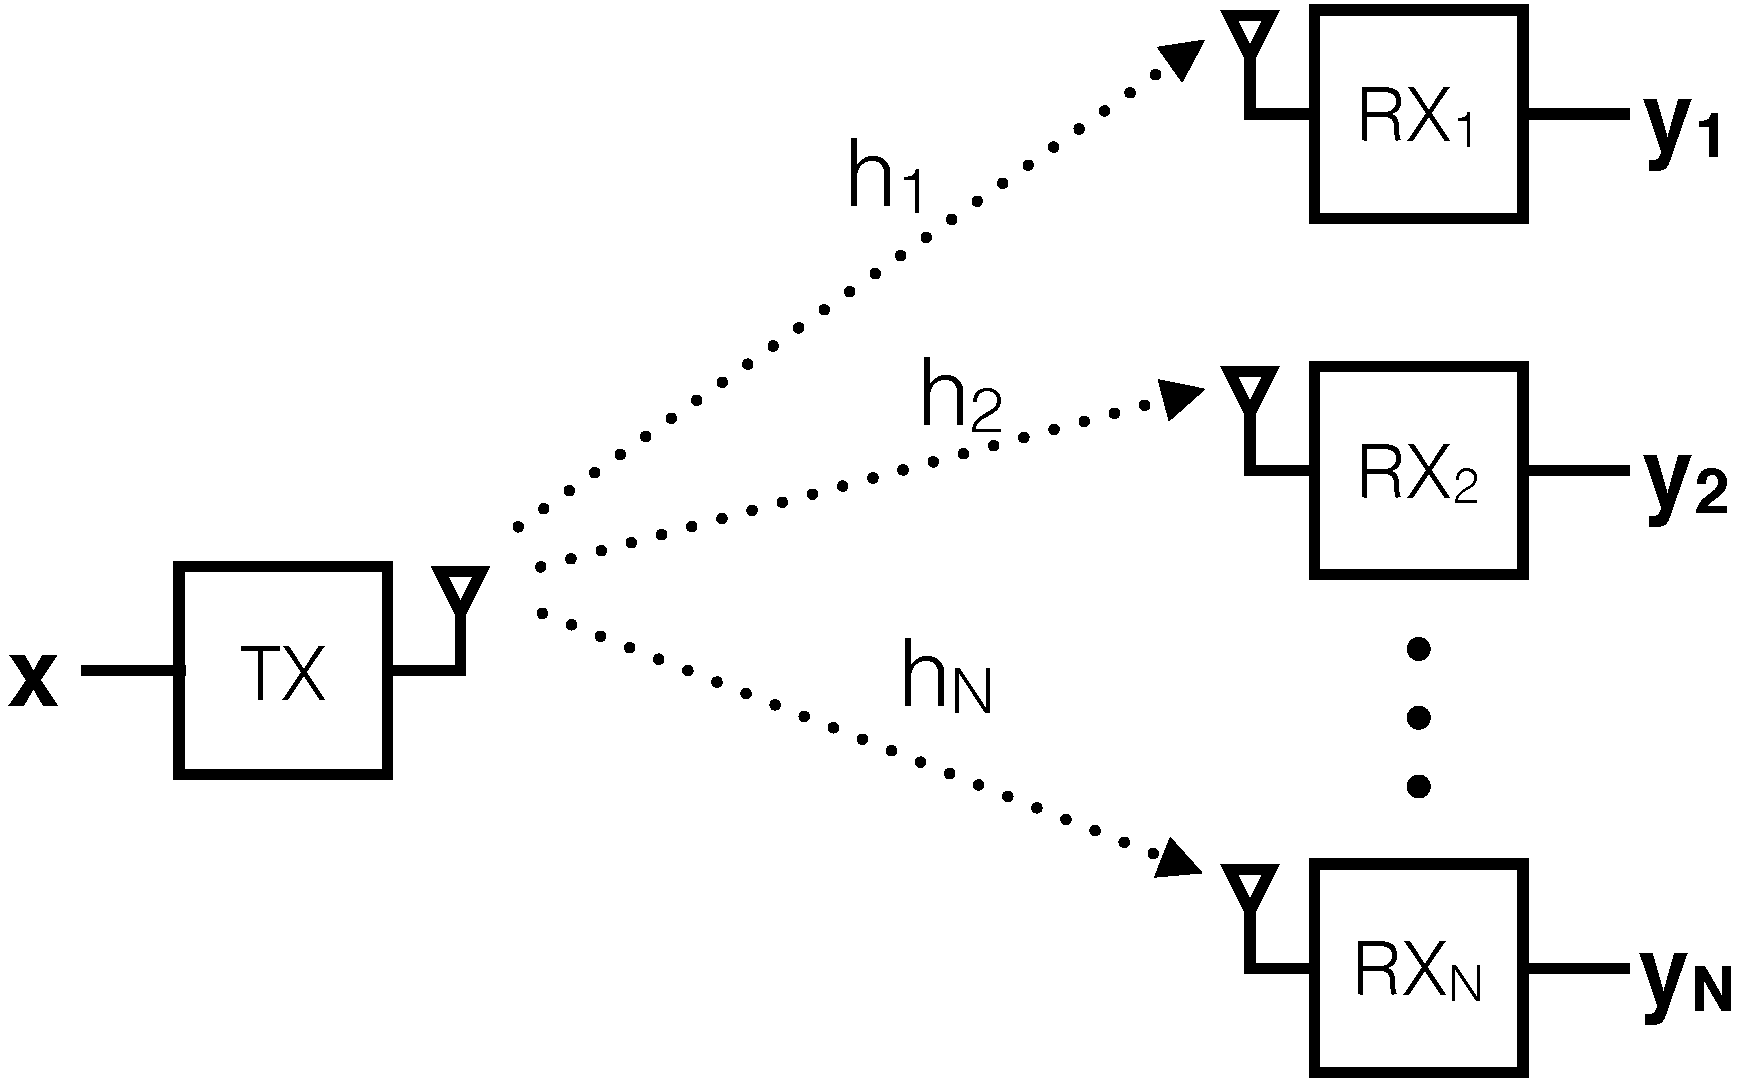
\includegraphics[height=1.25in]{figures/SIMO_cropped}
    \vspace{-10pt}
    \caption{Coherent combining helps receivers collaboratively improve
        signal-to-noise ratio}
    \label{fig:simo}
    \compactimg
\end{figure}

Wireless radios leverage multiple antennas (MIMO or multiple-input
multiple-output) to improve throughput. This paper considers coherent
combining where transmissions from a single-antenna transmitter (e.g. an
LPWAN client) are heard by multiple receiver antennas (e.g. LPWAN gateways).
These gateways can then coherently combine the received signals to improve
signal decodability.

Mathematically, let the transmitted signal be $x$ and each of the gateways
receive a signal $y_i$ through wireless channel $h_i$, introducing an
independent noise $n_i$ at the receivers. For a narrow-band system (as is
LoRaWAN and most LPWAN technologies), we can write the received signal as:
$y_i = h_i x_i + n_i $.

The receivers can now coherently combine their received signals by using the
known wireless channels $h_i$:

\compactimg

\begin{align*}
y_{\text{combined}}
	= \sum_{i=1}^N h^*_i y_i
	= \sum_{i=1}^N \left| h_i \right|^2 x + \sum_{i=1}^N h^*_i n_i
\end{align*}

The first term is the combined signal while the second term is the combined
noise. However, while the signals add up coherently, the noise, being
independent, adds up incoherently. This results in an overall increase in the
combined SNR, which allows us to jointly decode a packet, that may otherwise
not be decodable by any individual receiver.

\compactimg

\begin{align*}
SNR_{\text{combined}} %= \frac{\text{total signal power}}{\text{total noise power}} 
	= \frac{\left| \sum_{i=1}^N \left| h_i \right|^2 x \right|^2}{\sum_{i=1}^N \left| h^*_i n_i \right|^2} 
	\geq \frac{\left| \left| h_i \right|^2 x \right|^2}{\left| h^*_i n_i \right|^2} = SNR_i
\end{align*}

In practice, performing coherent combining as shown above makes two important
assumptions: (1) the packets can be detected at individual receivers above
some SNR threshold, and (2) receivers share a common clock reference for time
and frequency. This paper describes the challenges in implementing coherent
combining in the low-power wide-area context where neither assumption holds.


\subsection{Primer on LoRaWAN PHY and MAC}
\label{sec:lora}

LoRaWAN is a popular LPWAN technology that operates in the sub-GHz ISM band
(900 MHz in the U.S.) and bandwidths of 125-500kHz. LoRaWAN clients can
transmit at low-data rates (few kbps) to gateways up to 10 km away in free
space and last up to 10 years on AA batteries. Below, we detail a few key
design decisions of LoRaWAN.

\noindent \textbf{LoRa, The PHY: } LoRa's physical layer is based on
chirp-spread spectrum modulation, i.e. using a chirp signal that continuously
varies in frequency. This makes it resilient to interference, multi-path
fading and doppler effects. Every LoRaWAN packet begins with a preamble of
sixteen repeated chirps followed by data. Each data chirp encodes multiple
data bits (more precisely, \textit{chips}), with the number of  bits encoded
per chirp called the \textit{spreading factor} (SF). For instance, at
spreading factor of seven, each chirp encodes 7 bits with $2^7 = 128$ possible
uniformly separated initial frequencies. A higher spreading factor, e.g.
eight, encodes one more bit per chirp but also incurs double the transmission
time, effectively halving the data rate.\footnote{More precisely, increasing
spreading factor from $n$ to $n+1$ scales data rate by $(n+1)/2n$.} Increased
spreading factors are used to simultaneously slow down transmissions and
improve resilience to noise. LoRaWAN radios are therefore designed to transmit
at the lowest possible spreading factor that can be received at existing noise
levels for minimizing transmission time and the resulting battery drain. This
paper therefore strives to reduce spreading factor (improve data rate) for
weak transmitters.

% \vspace*{0.02in}

\noindent \textbf{The MAC: } LoRaWAN networks are designed to be simple
star-topologies that have client devices directly communicating with a gateway
that is connected to the internet over ethernet or cellular links. Gateways
are simple and relatively inexpensive forwarders that send received packets to
a cloud LoRaWAN server, and can be commanded by the server to transmit data to
clients at a specific time. Packet decoding, managing acknowledgements and MAC
parameters like data-rate are decided at a LoRaWAN server. The LoRa community
often refers to the system as having a ``MAC-in-the-Cloud'' design. LoRaWAN
allows and encourages its users to deploy their own gateways. These gateways
are completely unplanned and on low-bandwidth, unreliable internet connections
(compared to cellular base-stations that are extensively planned and have
dedicated optic fiber connections). In this paper, we refer to these as
user-deployed gateways. The penultimate goal of this paper is to make
individual unreliable user-deployed gateways more valuable by pooling together
PHY-layer processing at the cloud.

\section{Charm's Architecture}
\label{sec:arch}

The goal of Charm is to decode weak transmissions, which cannot be decoded
by any individual gateway, by collating receptions from multiple gateways at
the cloud. At one level, this  enables us to expand network coverage area
reaching clients deep inside buildings, underground or in outer reaches of the
city. More fundamentally, it saves energy on the vast majority of client
devices, even if they are within range of some gateways by allowing them to
increase their data rate without experiencing any loss in performance. Our
results in Sec.~\ref{sec:energy-savings} demonstrate that lowering transmit
time results in a direct and significant impact on battery life.

Fig.~\ref{fig:architecture} depicts Charm's architecture where we assume the
gateways can be user-deployed  both indoors and outdoors, at a cost of a few
hundred dollars. These base stations have an Ethernet backhaul to the cloud
that accommodate a maximum uplink bandwidth of a few megabits per seconds.
Much like the standard LoRaWAN architecture, MAC-layer scheduling is performed
at the cloud with gateways relaying their received data to the cloud. However,
to accommodate decoding weak received signals, we also allow gateways to ship
raw received I/Q signals from feeble low-power clients to the cloud. The cloud
aggregates such weak signals and coherently combines them to decode the
underlying data bits from feeble receptions across multiple gateways. In other
words, Charm performs a joint optimization of the  PHY-layer at the cloud,
simultaneously improving battery life and range of low-power clients at the
expense of increased computation at the cloud.

Realizing a scalable and real-time system based on the above architecture
is challenging both at the gateways and the cloud:
\begin{itemize}
\item {\bf At the Gateway: } Given that signals from weak LPWAN
clients are often well below the noise floor, gateways are unaware of these
packets in the received signal. This means that base stations must effectively
send all their received raw signal data to the cloud to detect and decode weak
signals, stressing their limited uplink bandwidth.
\item {\bf At the Cloud: } The cloud must identify signals from which
gateways need to be combined to recover transmitted data from multiple
clients. At city-scale, it is conceivable that overlapping weak transmissions
from different clients are received at the same time by gateways, making data
recovery challenging at the cloud. Additionally due to the use of low-cost
hardware that lacks precise time synchronization, each of the gateways adds
clock and frequency errors to the captured signals. These must be resolved
before the signals can be combined.
\end{itemize}

\begin{figure}[!htb]
    \centering
    % \vspace{-10pt}
    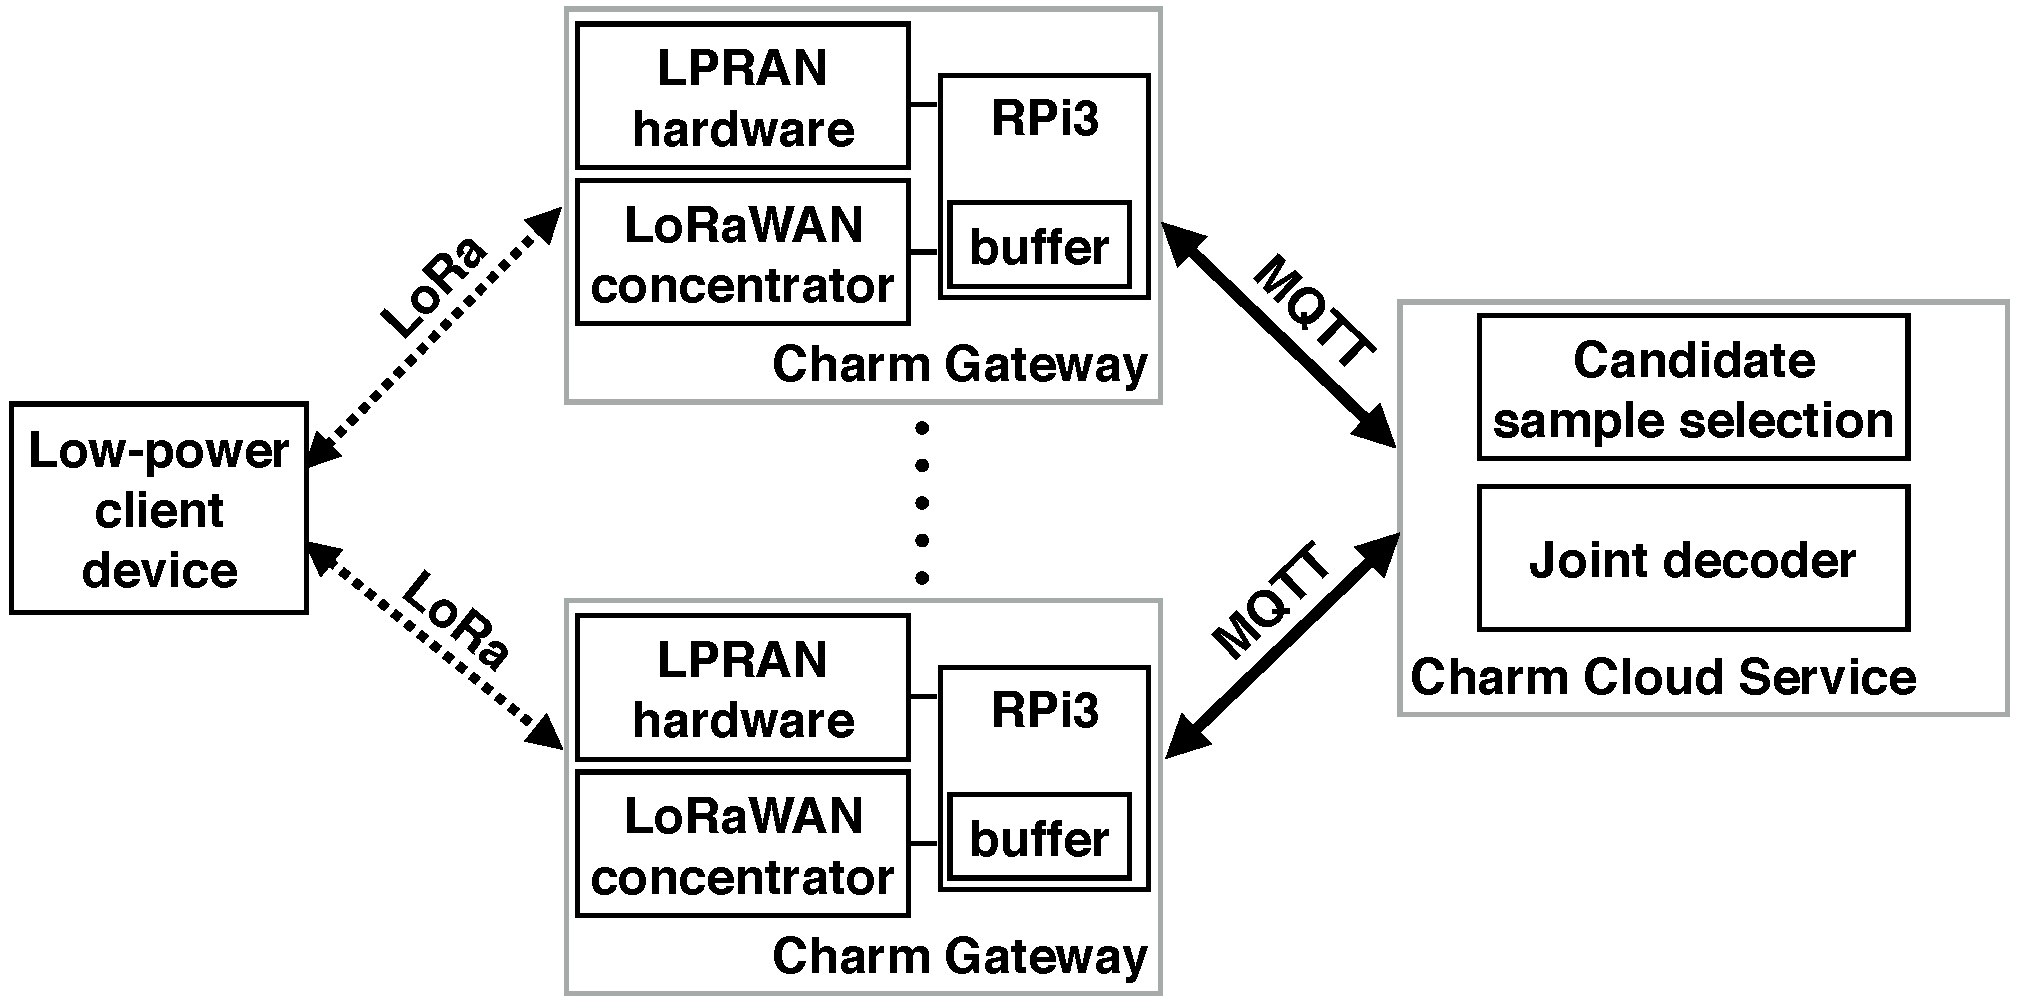
\includegraphics[width=0.45\textwidth]{figures/charm-architecture_cropped.pdf}
    \vspace{-10pt}
    \caption{Architecture of Charm}
    \label{fig:architecture}
    \vspace{-20pt}
\end{figure}

The rest of this paper describes Charm's solutions to each of these
challenges. Specifically, Charm makes two key contributions: (1) A software
interface at the gateway to identify weak transmissions to ship to the cloud,
and a hardware design that facilitates these decisions in real-time; (2) A
scalable cloud based PHY-layer processing system at the cloud that can operate
at city-scale. Next we elaborate on each of these components.
\section{The Charm Gateway}
\label{sec:gateway}

% {\color{blue} Points to cover
% \begin{itemize}
%     \item Hardware + block diagram + capability + how to decode IQ streams
%     \item Local detection algorithm
%     \item Optional: (LoRa-aware) compression
% \end{itemize}

% }

We first describe Charm's design at the gateway to enable accurate decoding of
weak clients, by relaying suspected weak signals to the cloud. Charm achieves
this first through a software algorithm at the gateway that identifies weak
transmissions that may be significantly below the noise floor. We further
implement this approach in hardware by building a custom programmable radio
platform for the gateway, that streams and processes raw I/Q samples using an
FPGA. We show how a Charm-gateway can detect weak signals in real-time through
this design, while simultaneously being programmable and responding to policy
changes from the cloud.

\subsection{Locally Detecting Weak Signals}
\label{sec:local-detection}

To reap the benefits of coherent diversity combining across multiple gateways,
Charm must relay weak signals to the cloud. Yet,
uploading all received signals to overcome this problem is
unfeasible given that gateways have limited uplink bandwidth to the cloud. To
put this in perspective, streaming all received I/Q samples to the cloud
requires an uplink bandwidth of 72 Mbps. However, the vast
majority of LPWAN gateways are likely to be user-deployed hardware such as
set-top boxes that cannot afford this bandwidth. Indeed, this creates
trade-off between detecting weak transmitters and conserving uplink
bandwidth.

Charm breaks this trade-off by detecting weak signals well below the noise
floor at a single LoRaWAN gateway. At a high level, our solution relies on the
structure of the LoRa protocol. Specifically, LoRa transmits signals in
the form of chirps, i.e. signals whose frequencies increase linearly in time.
In addition, several of these chirps are identical. For instance, consider the
initial preamble  in LoRaWAN with as many as 16 identical and consecutive
chirps. This means one can design a receiver that coherently sums up adjacent
symbols of any received signal over a sliding window. If the summing-up
operation is truly coherent, the underlying signal (i.e. the chirp) will add
up constructively, while noise will add up incoherently. In effect, this
boosts the signal-to-noise ratio of the received signal significantly,
allowing us to detect at least the preamble of a LoRaWAN packet. One can then
deliver a long chunk of packets surrounding this preamble to the cloud.

However the resolution of the above approach is a function of preamble length
-- the longer the preamble sequence is, the greater will be the extent of
noise that Charm can tolerate. Transmitting extremely long preambles increases
the overhead of the communication system, and in the long term, impacts
battery life. Charm therefore develops an approach that can detect weak
signals by leveraging data symbols in addition to the preamble -- even though
the transmitted data sequence is unknown a priori at the gateway. We detail
our approach below.

\noindent \textbf{Leveraging the structure of LoRaWAN data: } Charm seeks to
use the structure of the data symbols in LoRaWAN to improve detection of the
packet in the presence of noise. Indeed, much akin to the preamble, the data
symbols of a LoRaWAN packet are also composed of a sequence of chirps. Unlike
the preamble though, LoRaWAN data is composed of a sequence of chirps with
different frequency-shifts based on the bits they represent. Assuming that the
underlying data in a message is completely unknown and arbitrary, this makes
looking for structure within the data challenging.


\begin{figure}
    \centering
    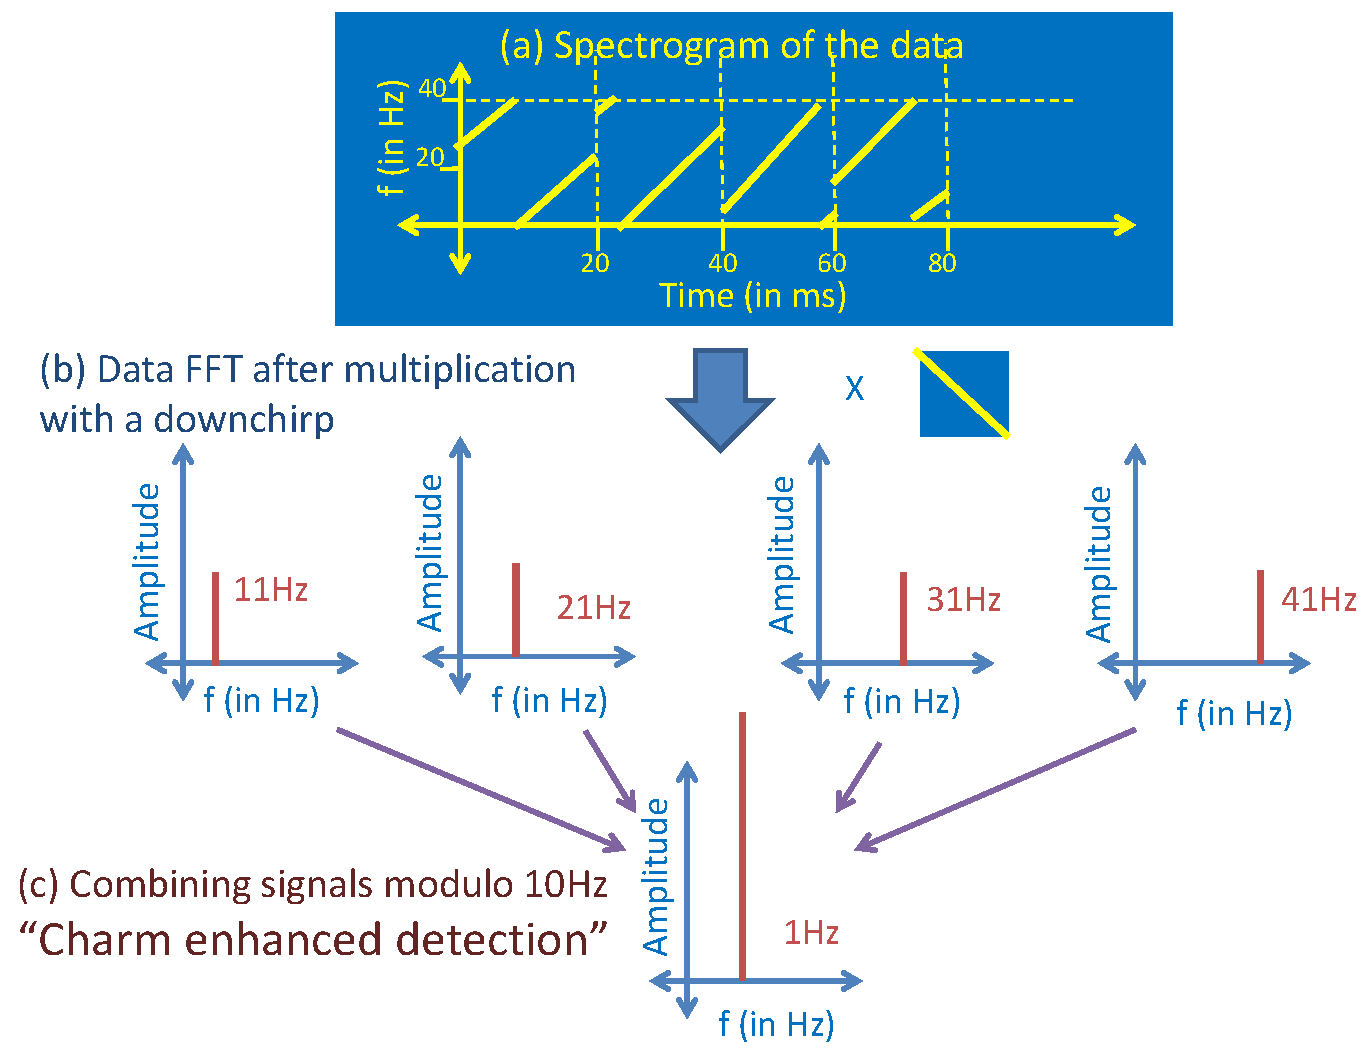
\includegraphics[width=0.85\columnwidth]{figures/CharmEnhancedDetection_cropped}
        \vspace*{-0.1in}
    \caption{The enhanced Charm packet detection process: The chirp signal (a)
    is multiplied by a downchirp in the Fourier domain (b). Windows of the
    resulting signal are then combined together (c) for threshold detection.}
    \label{fig:enhanced_charm}
    \compactimg
\end{figure}

Charm relies on the fact that while the data does cause shifts in frequencies
of chirps within the packet -- these shifts are not completely random. In
particular, chirps can undergo a discrete number of possible shifts based on
the number of bits per chirp. For a spreading factor of $SF$ (i.e. a
transmission data rate of $SF$ bits per chirp), the frequency shift is one of
$2^{SF}$ values. Charm therefore implements a solution that coherently
reinforces adjacent chirps, modulo the minimum possible frequency shift
between them. This ensures that regardless of their underlying data, adjacent
chirps always add up to reinforce each other while noise adds up destructively
as before. Given that there are a significantly larger number of data symbols
when compared to preamble symbols in any transmission, this provides an
additional mechanism to detect packets below the noise.

Mathematically, let $y_1, y_2, \dots, y_m$ denote the $m$ received data
symbols and $x_1, x_2, \dots, x_m$ denote the transmitted data bits encoded as
frequency shifts, each a number between $0$ and $2^{SF-1}$ where $SF$ is the
spreading factor. Let $\delta f = \text{Bandwidth} / 2^{SF}$ denote the
minimum possible frequency separation between two encoded data chirps.  Then
we can write the received signal at any time $t$ of the $i^{\text{th}}$ symbol
as:
\begin{align}
    y_i(t) = h e^{j 2 \pi (f(t) - x_i \delta f) t} + n_1 \label{eqn:yi}
\end{align}
Where $f(t)$ denotes the time varying frequency of the chirp, $j$ is the
square root of $-1$, $h$ represents the wireless channel and $n_i$ represents
noise.

When multiplied by $e^{-j 2 \pi f(t) t}$ and viewed in the Fourier domain,
this results in a single tone at frequency $x_i \delta f$ subject to noise.
Clearly the location of the tone is a function of the underlying data -- a
different quantity for different data symbols.

In contrast, let us sub-sample the above equation at times $t$ that are
multiples of $1/\delta f$ (let's say $t = \frac{k}{\delta f}$ for integer
values of $k$).

\begin{align}
    y_i\left(t\right) = h e^{j 2 \pi (f(t) - x_i \delta f) \frac{k}{\delta f}} + n_1 = h e^{j 2 \pi f(t) t} + n_1\label{eqn:yi2}
\end{align}
This time, when multiplied by $e^{-j 2 \pi f(t) t}$ and viewed in the Fourier
domain, this results in a single tone at frequency $0$ (subject to noise)
regardless of the underlying data in each symbol. In other words, sub-sampling
in the time domain led to aliasing of all the data peaks in the frequency
domain into one frequency bin (in this case, the DC bin), while noise is
smeared uniformly across all bins. Indeed, Charm repeats the sub-sampling
across multiple time steps separated  by $\frac{1}{\delta f}$ and averages the
results. The resulting average reinforces peaks corresponding to all the data
symbols coherently in one Fourier frequency bin, while noise adds up
incoherently among all remaining bins. This leads us to a very natural LoRaWAN
packet-detection mechanism that applies this operation across different
sliding windows of the received signals. We signal the presence of a packet
once our algorithm detects a significant peak in the Fourier domain that
dominates other peaks (subject to a threshold). Given that our approach
averages results over a large number of data symbols, it remains resilient to
noise without making assumptions about the contents of the packet itself.

\RestyleAlgo{boxruled}
\LinesNumbered
\begin{algorithm}[ht]
\caption{Charm's enhanced detection algorithm}
\label{alg:algorithm-label2}
 \For{bits in instream}{
 [C=I+jQ]=downsample(bits)\;
 \For{chirp\_length in C}{
    F=chirp\_length$*$down\_chirp\;
    FCollect.collect(F)\tcp*{Data Collection} 
 }
 C=FCollect.modulo($\delta f$)\tcp*{Modulus Bucketing}
 \If{$\frac{max(abs(fft(C)))}{mean(abs(fft(C)))}>\tau$}{
    SEND C to CLOUD \tcp*{Packet Forwarding}
 }
 }
\end{algorithm}

\noindent \textbf{Mitigating Frequency Offsets: } To add up signals from
adjacent symbols coherently, Charm must assume that the received symbols in
these signals are identical -- subject to noise and discrete shifts in
frequency due to the data (as described above). In practice however, wireless
signals from the LPWAN client to the gateway experiences an additional
arbitrary shift in frequency due to Carrier Frequency Offset (CFO). CFO stems
from the subtle variation in frequency between the clocks on the transmitter
and receiver. Given that the client is inexpensive, its clock often exhibits
large and arbitrary frequency differences relative to the gateway.
Additionally, the CFO for a given transmission received at different gateways
is also different and must be resolved individually.

Two properties of CFO make its impact on Charm's algorithm above particularly
damaging: (1) CFO unlike data introduces a frequency shift that is not
discrete, but continuous. As a result, it is not simply eliminated by looking at
the chirp in the Fourier domain ``modulo $\delta f$''  akin to the data as
described above. (2) CFO introduces a continuous phase shift $2 \pi
\Delta f_{CFO} t$ onto the received signal that accumulates over time. This
means that even otherwise identical received symbols may add up incoherently
owing to a time-varying phase shift.

The straw man approach to eliminate CFO would be an attempt to directly
estimate it. For instance, one could rely on the repeated symbols of the
preamble where any phase variation is purely a function of CFO. In particular,
the phase shift between two otherwise identical preamble symbols separated by
$t$ is simply $2 \pi \Delta f_{CFO} t$, which one can solve for to estimate $\Delta
f_{CFO}$ and eliminate its effect. However, this solution fails if the number of preamble symbols in the transmitted signal is insufficient to overcome noise. Further, this approach cannot exploit data symbols to estimate CFO, which, as explained earlier, are greater in number and would greatly enhance resilience to noise.

Charm overcomes this problem by realizing that while estimating $\Delta
f_{CFO}$ from the data symbols alone is challenging, it is sufficient to
estimate $\Delta f_{CFO}$ modulo $\delta f$ to detect the LoRa packet. To see
why, recall that the frequency offset over a packet $\Delta f_{CFO}$ can be
decoupled into two components: $[\frac{\Delta f_{CFO}}{\delta f}]\delta f + \{\frac{\Delta f_{CFO}}{\delta f}\}\delta f$, an
integer multiple of $\delta f$ and the remaining fractional component
respectively. When looking at the data chirps in the frequency domain modulo
$\delta f$, all the data symbols appear identical given that all frequency
shifts of the data are all multiples of $\delta f$. Similarly, the first term of the CFO:
$[\frac{\Delta f_{CFO}}{\delta f}]\delta f$ is also an integer multiple of $\delta f$ and therefore disappears under the modulo. Only the fractional part of the CFO: $\{\frac{\Delta f_{CFO}}{\delta f}\}\delta f$ persists
and introduces a time varying phase shift of $2 \pi \{\frac{\Delta f_{CFO}}{\delta f}\}\delta f t$
across symbols. This means that we can simply solve for the fractional component of CFO and eliminate its effect akin to the straw man approach, but using the data
symbols in the frequency domain modulo $\delta f$. In other words, Charm's
solution remains resilient to frequency offset, both in detecting the preamble
as well as data symbols of a LoRaWAN packet.

\subsection{Programmable Hardware Design}
\label{sec:hardware}

Charm must process raw I/Q samples from the gateway and selectively relay this
information to the cloud in real-time. However, existing LoRaWAN gateway
hardware cannot provide the raw I/Q streams necessary for joint decoding. In
contrast, deploying a full software-defined radio (SDR) at the gateway allows
packet decoding, it comes with high cost in term of power, sensitivity and
unit price. We therefore develop a custom Charm hardware platform shown in
\figref{lpran-hardware-images} as an auxiliary peripheral to a gateway and can
provide the necessary quadrature streams. Key to our performance is a
light-weight, low-cost and easy-to-reprogram hardware accelerator for data
reduction enabling further local processing (e.g. on the accelerator or by a
Raspberry Pi). In effect, we allow for a system that simultaneously allows
some SDR-like programmability of the PHY while maintaining high performance
and low cost.

\noindent  {\bf Compressing the Data Stream: } The raw IQ stream would be too
much for a low-power microprocessor, and  also contain too much redundant
information for our purpose. In particular, we use the SX1257 RF front-end
that provides 1-bit delta-sigma modulated signals at a whopping 36 MSps each
for the I and Q streams.  In order to keep the data stream to a more
microprocessor-friendly load, the design would require some lossless
compression. Through careful choice of parameters, we chose to compress the IQ
stream by summing consecutive samples in windows of size 64 and convert it
into a single 7-bit sample:
\begin{equation}
x_i = \sum_{j=64*i}^{64*i + 63} s_j
\end{equation}
, where ($x_i$) is the analyzable samples, and ($s_j$) is the I/Q sample
rates. A window size of 64 is selected since we are only interested in a final
bandwidth of approximately 500 kHz that the RF front-end is capable of
capturing. Upon applying the above technique, the compressed I/Q streams
generate data at a rate of 9 Mbps, down from the original 72 Mbps.

\begin{figure}[t]
\centering
\begin{tabular}{@{}c@{}}
\subfloat[Block diagram of the Charm programmable radio hardware platform]{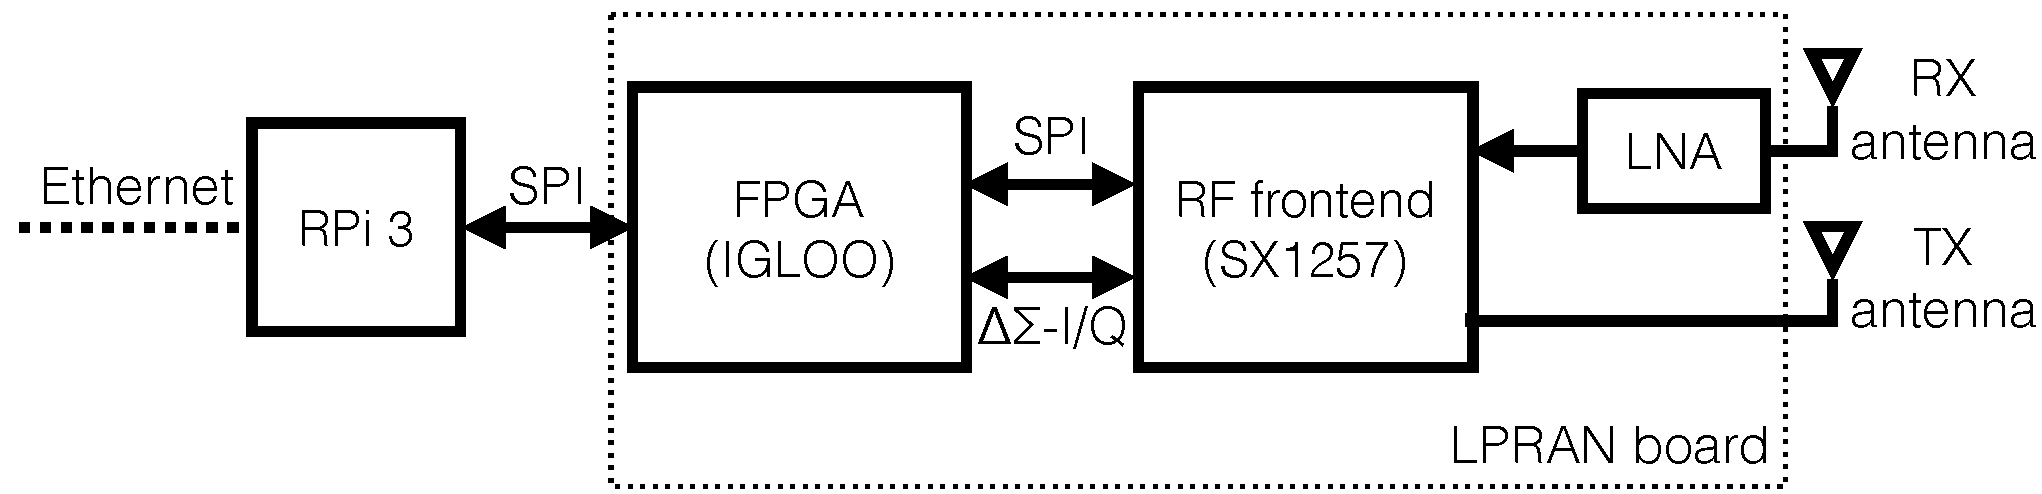
\includegraphics[width=0.40\textwidth]{figures/lpran-block_cropped}
\label{fig:lpran-block}} \\
\subfloat[Charm programmable gateway]{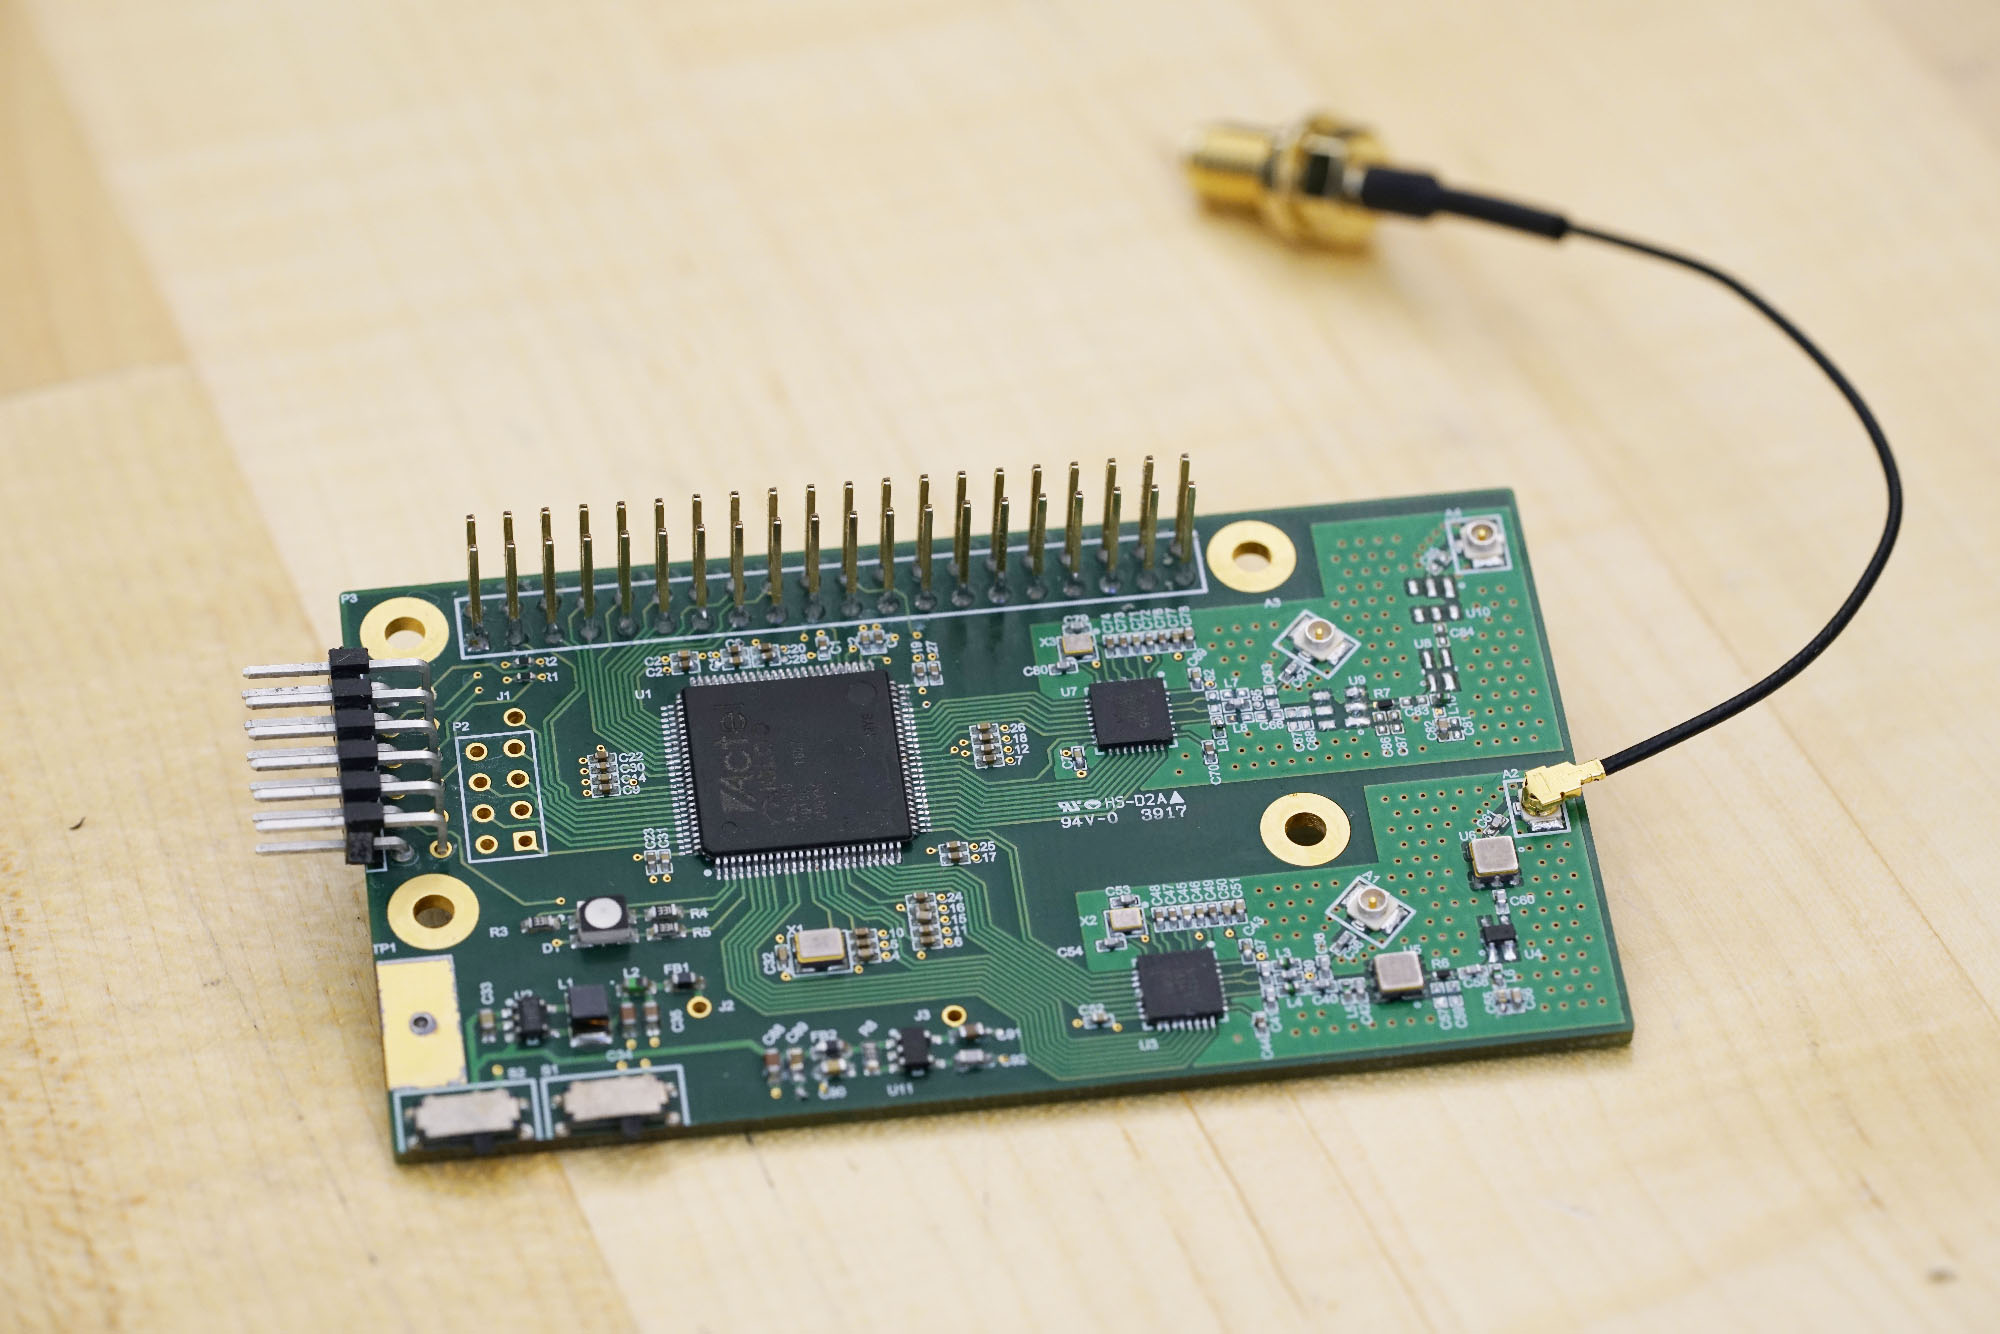
\includegraphics[width=0.23\textwidth, height=1.2in]{figures/gw-anon-sm}
\label{fig:gw-pcb}} 
\subfloat[Gateway with Charm hardware and LoRaWAN~concentrator]{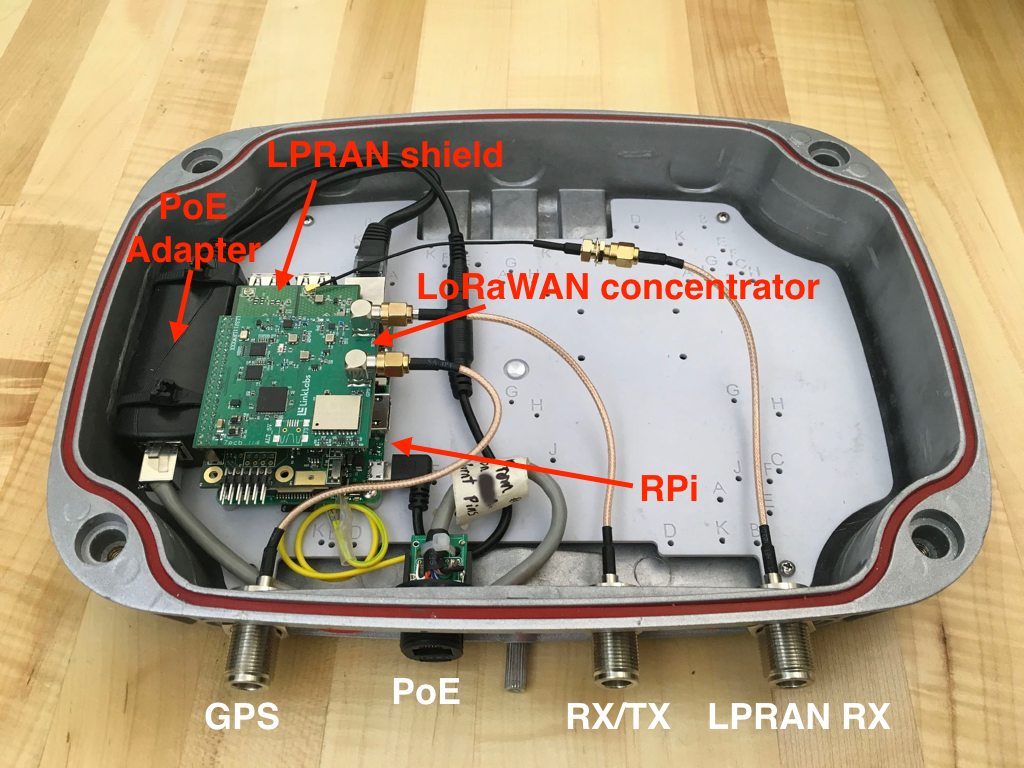
\includegraphics[width=0.23\textwidth, height=1.2in]{figures/annotated_gateway}
\label{fig:gw-annotated}}
\end{tabular}
\vspace*{-0.1in}
\caption{Charm Hardware Platform}
\label{fig:lpran-hardware-images}
\compactimg
\end{figure}

\noindent  {\bf Programmability: } The delta-sigma I/Q samples are processed
locally on a Microsemi IGLOO AGL250 FPGA, which performs the necessary
compression for data reduction.   The stream of data is transferred using a
high-speed serial interface (SPI) to the microprocessor (Raspberry Pi), and
forwarded when requested by the joint-decoder for additional processing. Each
block of samples are double buffered to ensure the validity of the data during
transfers. The microprocessor can then perform additional local processing,
time-stamping and temporary local storage until a stream is requested by the
joint-decoder. While our hardware platform is not a full-scale SDR, the FPGA
allows programmers to implement advanced real-time algorithms for packet
decoding and/or full duplex transmission across multiple channels. In
addition, the Raspberry Pi allows for ease of programmability when gathering
low-rate statistics about the received signals at the gateway. Overall, we
believe the Charm hardware platform will reduce the barrier for LPWAN
PHY-layer innovation for programmers and researchers across the board.
\section{Charm in the Cloud}
\label{sec:cloud}

At the cloud, Charm seeks to coherently combine received signals from multiple
gateways to recover weak received signals. At a high level, Charm collates I/Q
samples from multiple gateways and estimates their packet start time and
wireless channel. It then uses standard coherent SIMO combining (see
Sec.~\ref{sec:simo}) of the same weak transmission across multiple gateways to
ensure that the data can be accurately recovered. Charm repeats this
cloud-based PHY-layer processing at city scale across clients and gateways.

The rest of this section describes the key challenges and opportunities in
making the above design scalable and practical. First, we describe Charm's
approach to ensure accurate time-synchronization between gateways -- showing
how even an offset of one or two samples can be severely detrimental to
coherent combining. Second, we present our solution to dynamically infer
signals from which gateways need to be combined over time to best recover a
weak signal. Finally, we present opportunities to improve bandwidth and system
performance at the cloud by avoiding wasted transmissions of I/Q data to the
cloud as well as wasted computation.

\subsection{Time Synchronization at the Cloud}
Charm relies on the accurate timing of received weak signals at the gateways
for two important reasons: First, any offset in timing between signals
corresponding to the same packet across  gateways will prevent the signals
from coherently combining. Second, the precise start time of packets across
gateways is valuable information to identify the packet, allowing Charm to
infer which received signals across gateways correspond to the same packet.

A naive approach to synchronize base stations would be to synchronize them
through highly accurate clocks (GPS-synced) or through time-synchronization
protocols in software over the backbone network (e.g. NTP). In practice, for
indoor gateways (e.g. set top boxes) connected to an Ethernet backhaul, these
can provide time synchronization of up to a few milliseconds. In practical
terms, this means that the received signals at the gateways can be time
synchronized to within a small number of time samples.

% \begin{figure}
%     \centering
%     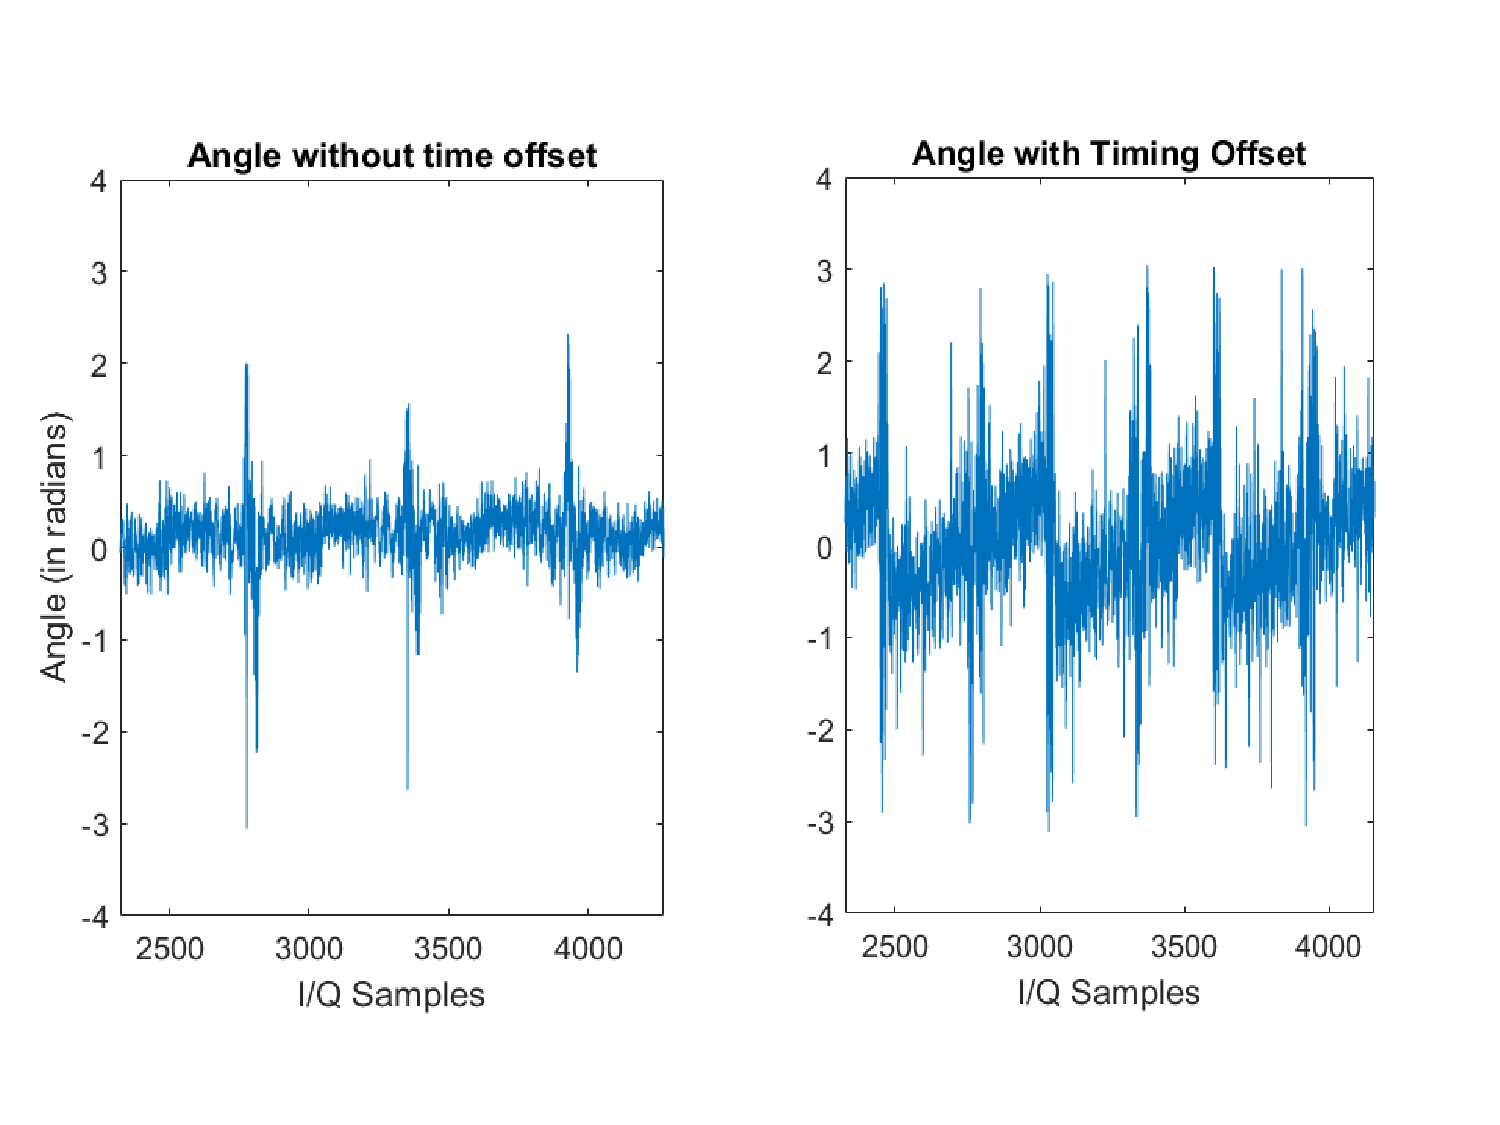
\includegraphics[height=1.6in]{figures/TimeOffset.pdf}
%     \vspace*{-0.1in}
%     \caption{Effect of timing offset on detection}
%         \vspace*{-0.0in}

%     \label{fig:toffset}
%     \compactimg
% \end{figure}

\begin{figure}[!htb]
\centering
\compactimg
\subfloat[Without timing offset]{
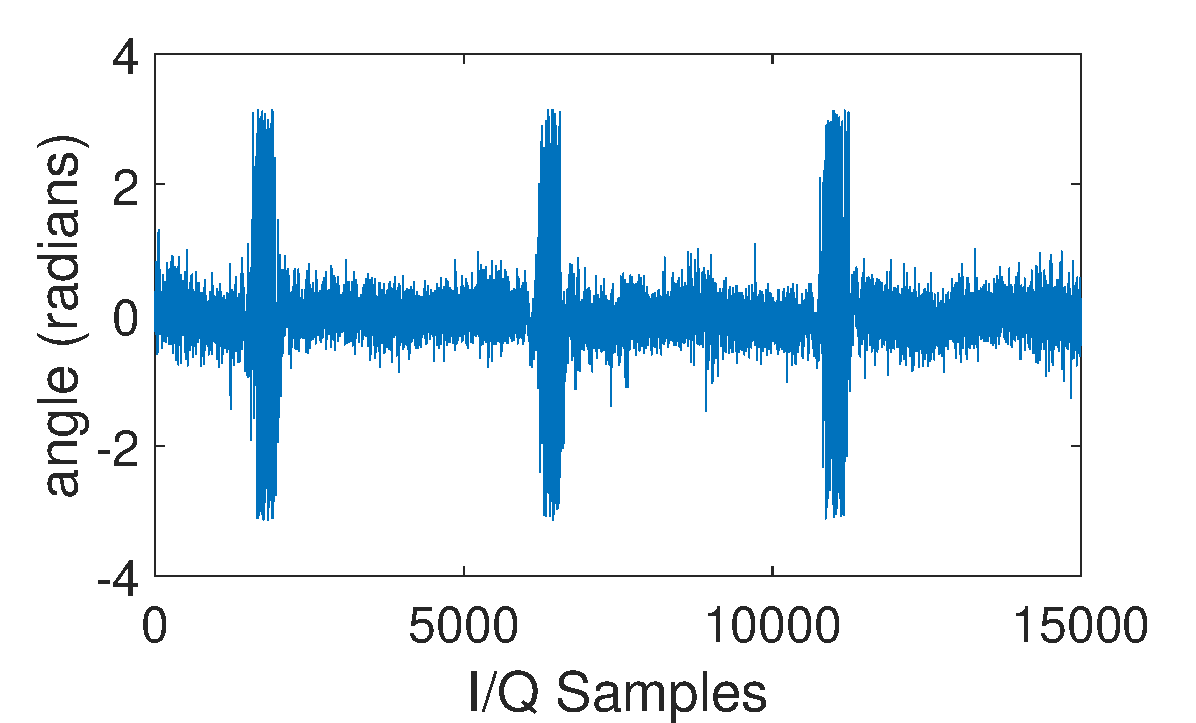
\includegraphics[width=0.48\columnwidth]{figures/detection_woOffset}
\label{fig:detection-wo-offset}}
\hfill
\subfloat[With timing offset]{
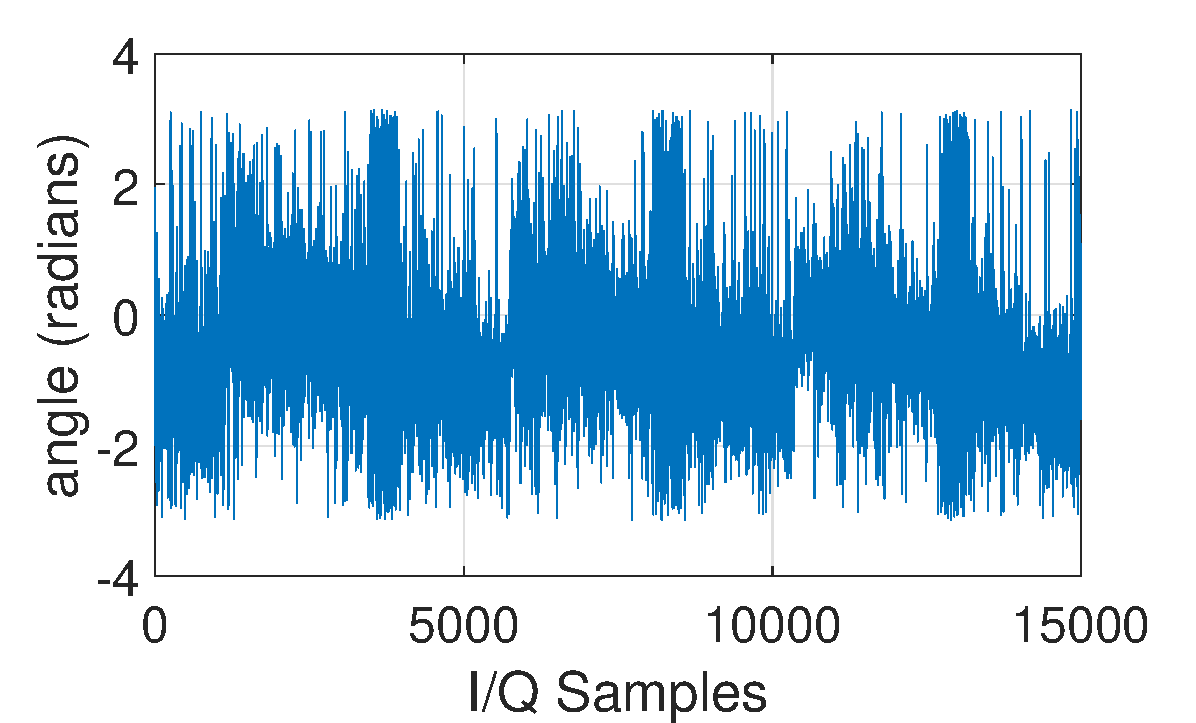
\includegraphics[width=0.48\columnwidth]{figures/detection_wOffset}
\label{fig:detection-w-offset}}
\vspace{-10pt}
\caption{Effect of timing offset on detection}
\label{fig:toffset}
\vspace{-10pt}
\end{figure}

Unfortunately, even a small offset in the timing between two gateways can
severely deteriorate coherent combining. Fig.~\ref{fig:toffset} depicts a
simple example of the phase difference between two gateways whose signals are
offset by zero and one sample respectively. We note that even an offset of one
frequency bin causes a significant time-varying error in phase between the
gateways. As a result, summing up these signals would cause some symbols
in-phase to reinforce, while others that are out-of-phase cancel each other.
\vspace*{0.1in}

\noindent {\bf Phase-Based Time-Sync Below the Noise Floor: } Charm overcomes this
challenge by recognizing that small time-errors between two gateways results
in a phase difference over time that is predictable. As shown in
Fig.~\ref{fig:toffset}, this phase difference is a linear function of time,
given by $2\pi f(t) \delta t$, where $f(t)$ is the instantaneous frequency of
the chirp (linear in time) and $\delta t$ is the required timing offset. In
principle, one can therefore estimate the slope in phase over time to recover
the timing offset. In practice however, doing so is challenging, particularly
when each received signal at each gateway is completely buried below the
noise. The phase of such signals at any such gateway simply appears to be
random -- making any form of linear regression of the slope highly
error-prone.

Charm overcomes this challenge using two key properties: First, owing to
coarse time synchronization of the gateways (via NTP), any residual timing
error between them is limited to a few samples. This allows Charm to
iteratively optimize over a small number of time-shifts to infer the offset
that leads to the best fit. Second, Charm's can extract timing offsets both
from the preamble and the data symbols. To see how, notice that our approach
only considers the {\it difference} in phase between the same packet heard at
two different gateways. Given that, in the absence of timing offsets, both
gateways perceive the same underlying message bits over time, the resulting
phase difference would be independent of the transmitted data bits -- whether
they belong to the preamble or data.

Charm's approach therefore considers a the range of possible small offsets
between any two received signal sequences. For each candidate offset, it
computes the phase difference between the signals as a function of time. It
then identifies the true offset between the gateways as the one whose phase
difference varies minimally across the entire packet. Given that our approach
averages measurements through the entire packet (both preamble and data), it
remains highly resilient to noise.\vspace*{0.1in}


\noindent {\bf Maintaining Synchronization across Packets: } Finally, Charm
can learn the time-offsets between gateways, particularly in busy urban
deployments, by using information from past packets. Recall that Charm's
coherent is only affected by timing errors between pairs of gateways -- not
the gateway and any particular client. While these errors may change over
time, over small intervals (e.g. hundreds of milliseconds), they are unlikely
to change. As a result, one can use the measured time offset from a previous
packet to infer the offset at the next packet that follows soon after. This
allows us to maintain a history of the time-offsets, smoothed by algorithms
such as Kalman filtering with outlier rejection, that helps us better predict
time offsets between gateways even when signals from certain clients are too
weak to measure these reliably.

\subsection{Joint Decoding at the Cloud}
\label{sec:joint-decoding-cloud}
This section answers an important question: How does Charm decide which weak
signals received from a set of gateways need to be combined coherently? In
other words, Charm must identify which signals at the gateway correspond to
the same packet from the same transmitter. It must do so even in the presence
of overlapping transmissions from multiple clients at geographically different
locations.

\noindent {\bf Which Signals Should We Combine?: } Charm addresses this challenge by
using the timing information of packets to infer transmissions that correspond
to the same user. It further uses the perceived signal-to-noise ratios and
geographic location of the gateways and measures the likelihood that far-away
gateways can listen to transmissions from the users at the observed
signal-to-noise ratios. It then calculates a feature vector for each received
signal that contains two tuple: (1) The time instance at which the packet was
received; and (2) The geographic location of the gateway. We apply the OPTICS
clustering algorithm~\cite{ankerst1999optics} to then cluster received signals
from multiple clients at any time instance.

Past-clustering, we combine received signals from a subset of clients in each
cluster. Specifically, we only choose to combine signals with a sufficiently
high signal-to-noise ratio. This is because transmissions that are highly
noisy tend to add little additional value yet cost uplink bandwidth.

An important consequence of our clustering approach based on geographic
location of the gateway is that it facilitates spatial re-use. Specifically,
it is quite possible that weak transmissions from two different neighborhoods
occur at the same time but are heard at distinct subsets of gateways. Charm
allows us to decode these transmissions simultaneously without mixing up their
signals. Indeed, gateways that are geographically in-between and hear
interfering signals from both clients can be simply weeded out from clustering
due to their poor signal-to-noise ratio.

\noindent {\bf Joint Decoding Algorithm: } Algorithm~\ref{alg:algorithm-label}
below describes Charm's joint-decoding algorithm end-to-end. At a high level,
our approach retrieves the wireless channels of the signals to be combined at
any instance, their timing offsets and frequency offsets computed as described
in the above sections. We, then eliminate any phase errors owing to time and
frequency offsets in the received signals. We then coherently sum up the
resulting signals multiplied by the conjugate channels as described in
Section~\ref{sec:background}.

\RestyleAlgo{boxruled}
\LinesNumbered
\begin{algorithm}[t]
\caption{Joint decoding algorithm}
\label{alg:algorithm-label}
 packets = receive\_data(candidates)\;
 \For{p in packets}{
 p = $e^{j2\pi (\Delta_f)t}$ p \tcp*{Freq Offset Correction}
 p = $e^{j2\pi f(\Delta_t)}$ p \tcp*{Timing Offset Correction}
 h(p)$=\frac{p}{reference}$ \tcp*{Channel Estimation}
 }
 combined\_packet$=$zeros(p)\;
 \For{p in packets}{
 combined\_packet = combined\_packet + h$^*$p \;
 }
 decode(combined\_packet)\;
 SEND ACK\;
 \end{algorithm}

\subsection{Opportunistic Fetching of Information}
Our design thus far assumes Charm gateways relay raw I/Q received signals to
the cloud, only if their signals are too weak to be decoded, yet can be
detected. However, this approach can be ineffective for two reasons: (1) On
the one hand, the cloud may have already received the decoded data bits from
another gateway, meaning that Charm simply wasted uplink bandwidth
unnecessarily; (2) On the other hand, some received signals may be
significantly below the noise floor even to be detected, yet be valuable
enough to be relayed to the cloud to be jointly decoded with other such weak
receptions.

\noindent {\bf Two-Phase Data Fetch: } Charm overcomes these challenge through
a pull based approach where gateways relay raw I/Q samples to the cloud, only
when explicitly asked for by the cloud. Each gateway keeps a circular buffer
of I/Q streams as well as any recent snapshots containing a potential packet.
For each potential reception, a gateway first reports its signature (center
frequency and spreading factor), the time of the reception packet, the
perceived wireless channel and signal-to-noise ratio. Charm then performs
clustering as described above and requests the raw I/Q samples {\it only }
from clients whose signals were chosen to be combined. Given that latency to
the cloud are of the order of few milliseconds, smaller than a typical LoRaWAN
packet size (tens, often hundreds of milliseconds), our system can perform
decoding virtually in real-time at LPWAN timescales, despite incurring
multiple round-trip times in fetching information.

\noindent {\bf Opportunistic Data Buffering: } In some instances, Charm's
clustering algorithm may fail to have enough signals to successfully combine
and decode a packet using the gateways that detected the packet alone.
However, Charm may be able to opportunistically fetch information from other
gateways in the same geographical region of the cluster and tuned to the same
frequency who may have received the same signal, yet at a signal-to-noise
ratio too weak to detect locally. Charm therefore requires all gateways to
store past signals for up to 1.6 seconds (maximum LoRaWAN packet length) in
the past in a 5 MB circular buffer. This allows Charm to query and fetch
signals from gateways, even in scenarios where only one gateway in the entire
network was able to locally detect a signal from a given transmitting client.
\section{Integration with LoRaWAN}
\label{sec:implementation}

\begin{figure}[t]
\centering
\compactimg
\begin{tabular}{@{}c@{}}
\subfloat[OpenChirp network coverage heatmap]{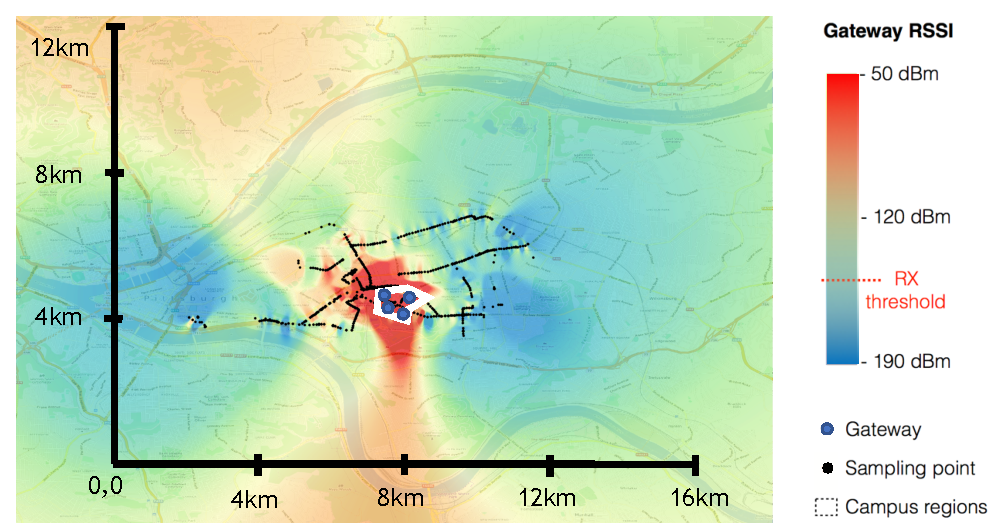
\includegraphics[height=1.2in]{figures/heatmap_openchirp_cropped}
\label{fig:coverage-map}}
\hspace{0.05in}
\subfloat[Rooftop gateway]{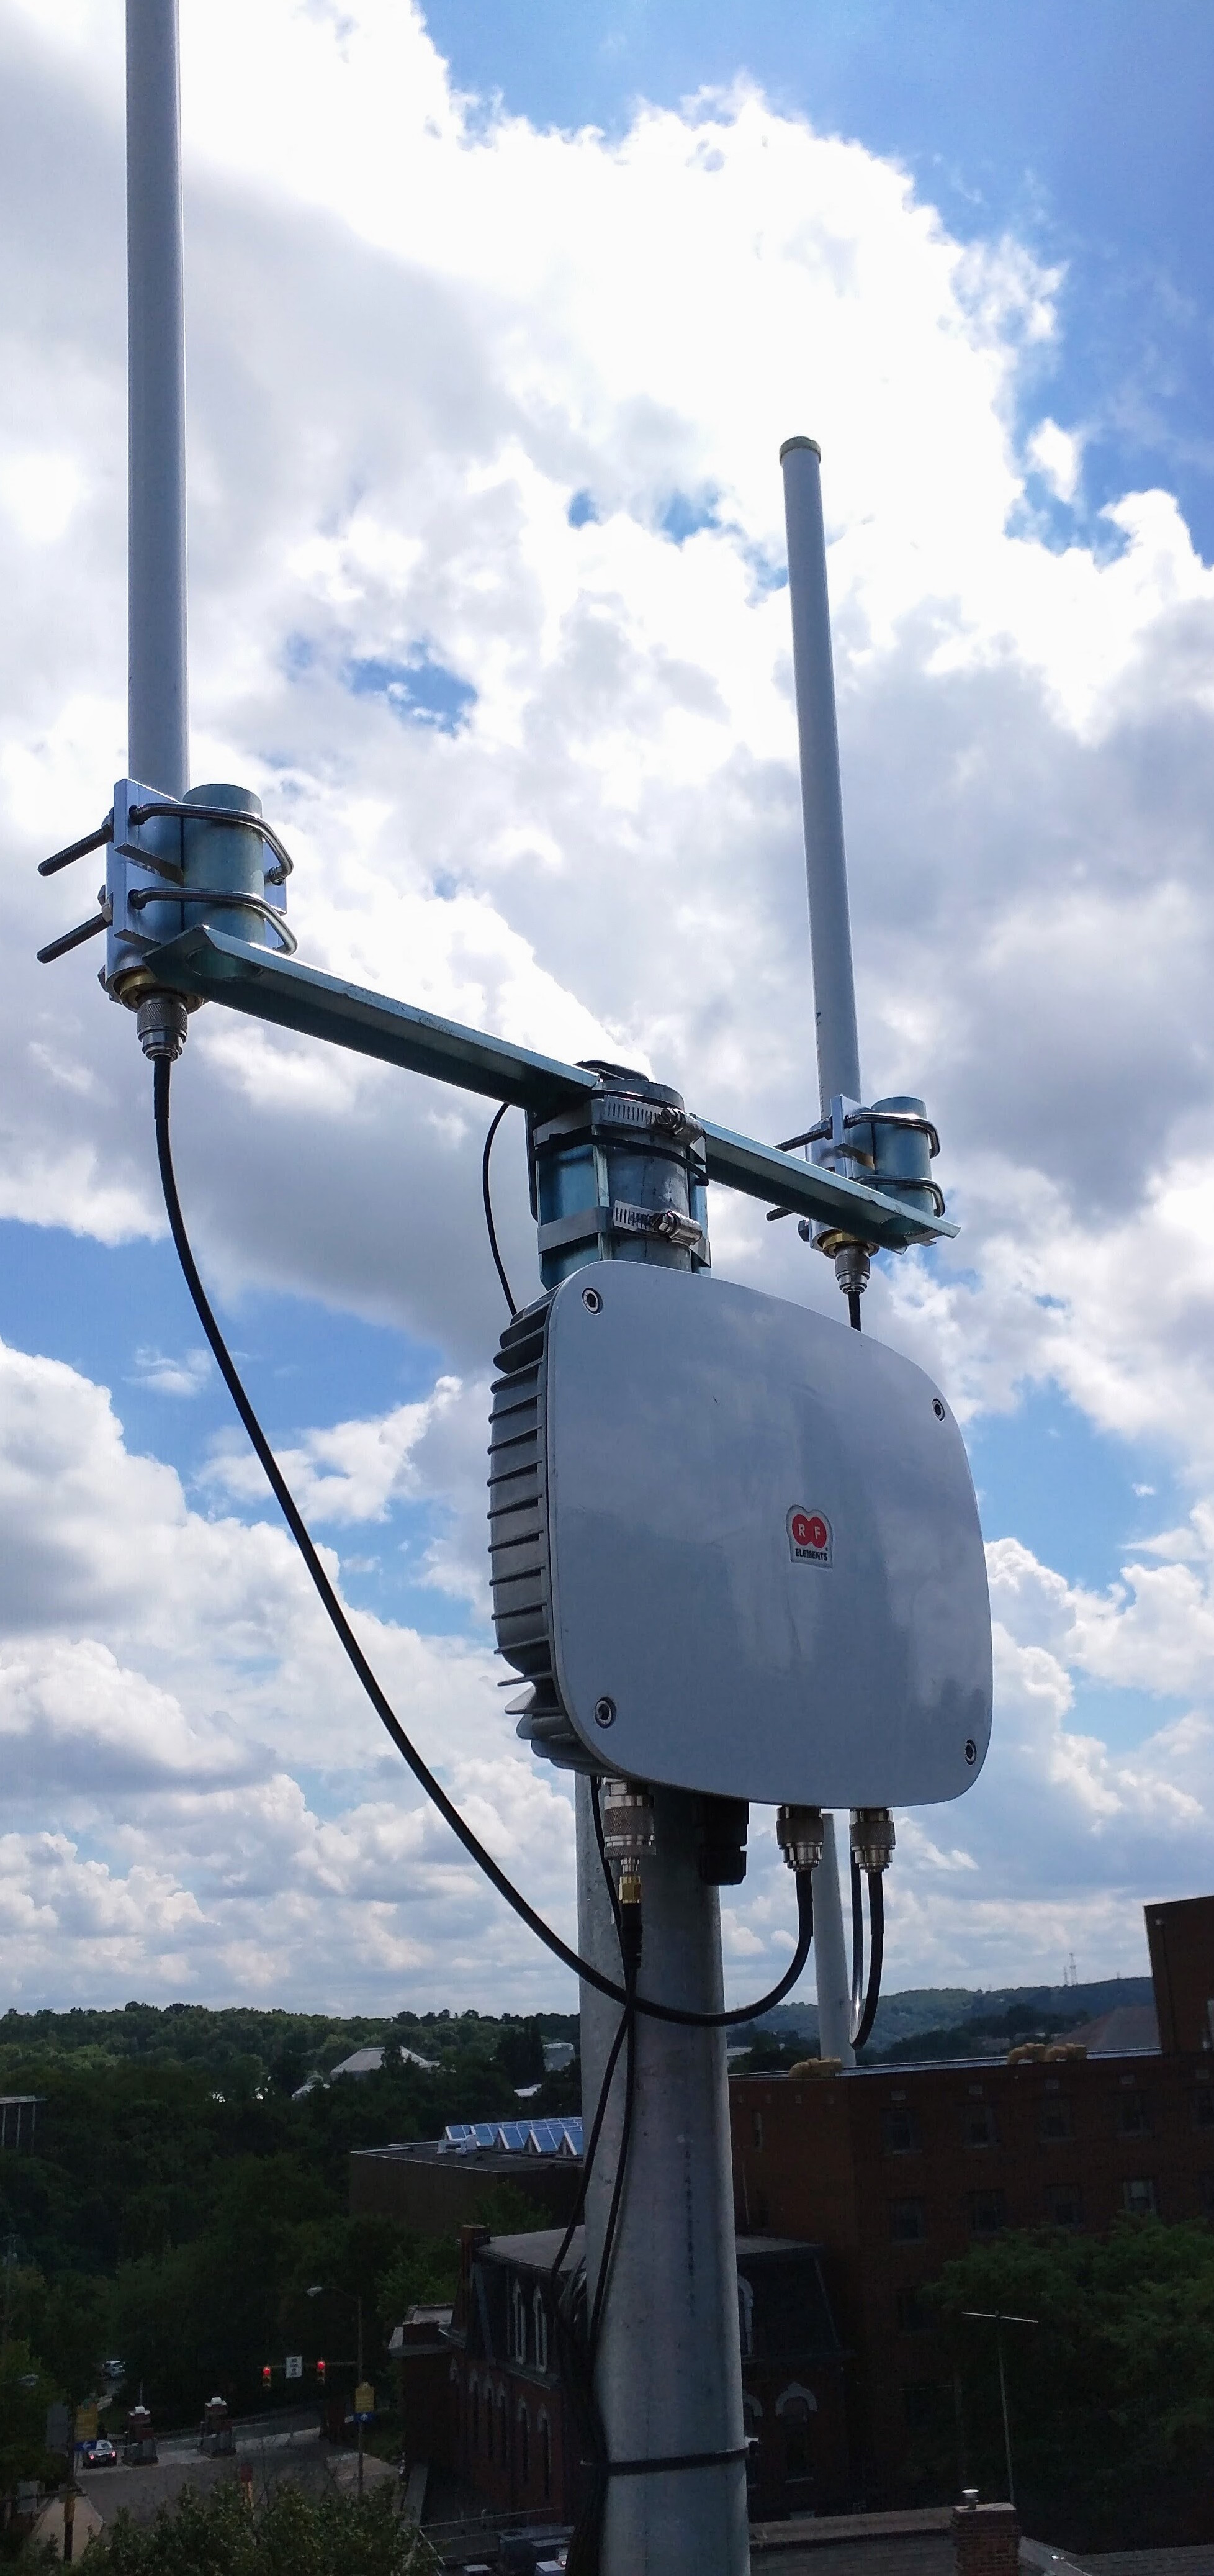
\includegraphics[height=1.2in]{figures/gateway_deployment_cropped}
\label{fig:rooftop-gw}}
\end{tabular}
\caption{Openchirp LoRaWAN deployment in Pittsburgh}
\label{fig:deployment}
\compactimg
\end{figure}

Charm is implemented as a service running on a campus-wide LoRaWAN network installed at Carnegie Mellon University.  We currently have four gateways mounted on rooftops providing wide area coverage and eight auxiliary indoor gateways extending coverage into remote parts of campus. The LoRaWAN network is powered by the open-source OpenChirp (\url{http://www.openchirp.io}) framework that allows students and faculty to login with their campus accounts and create device endpoints for capturing and sharing data.  OpenChirp provides services that can be attached to data streams that can perform operations ranging from basic data storage to binary-to-JSON packing and unpack. A RESTful interface is used to configure meta-information about devices and set access control privileges that define how other users can interact with data streams.  The only modifications required to make a gateway Charm enabled is the additional hardware platform for receiving raw I/Q streams and a modified LoRaWAN packet forwarder that runs the packet reception event detector, maintains a circular buffer of I/Q streams and brokers interactions with the Charm cloud.  Communication between gateways and the cloud is managed using the OpenChirp's MQTT publish subscriber messaging layer where compressed Charm packets can be easily grouped and organized based on location.  The Charm service can instruct clients to switch to faster data rates (as compared to the normal data rate negotiation process) by spoofing improved SNR values during the join process. In this way, Charm can seamlessly operate with existing LoRaWAN devices with no modification.



\figref{deployment} shows examples of our gateway hardware deployed in the field along with the coverage in and around campus.  The network is currently supporting a wide-range of applications from student projects, study-space monitoring, and building occupancy sensing all the way to mechanical room environmental sensing and utility sub-metering for the campus facilities maintenance team.  The client transmitters in our experiments use the Semtech SX1276 LoRaWAN chipset. The figure also shows an example coverage heat map generated by nodes deployed throughout campus and the neighboring area.  We see that the network with just four outdoor gateways is able to cover almost 10$km^2$ of urban space.


\begin{figure}[hbt]
\centering
\begin{tabular}{@{}c@{}}	
\subfloat[Typical client device current consumption for a complete LoRaWAN transmission. The device is powered at $3V$.]{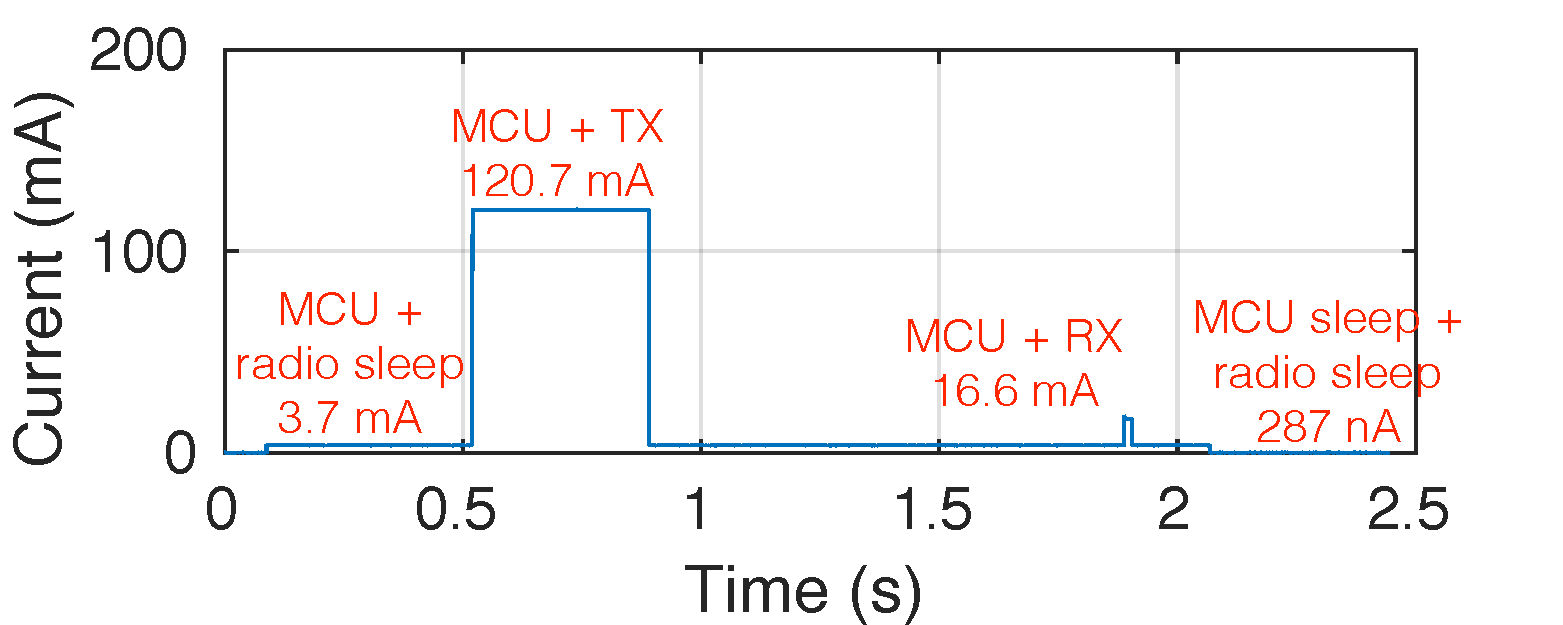
\includegraphics[width=0.36\textwidth]{figures/bug_power_trace_annotated}
\label{fig:power-trace}}\\
\hspace*{0.1in}
\subfloat[Estimated lifetime of a client device powered by two AA batteries sending 36 byte packets at various data rates based on the energy profile.]{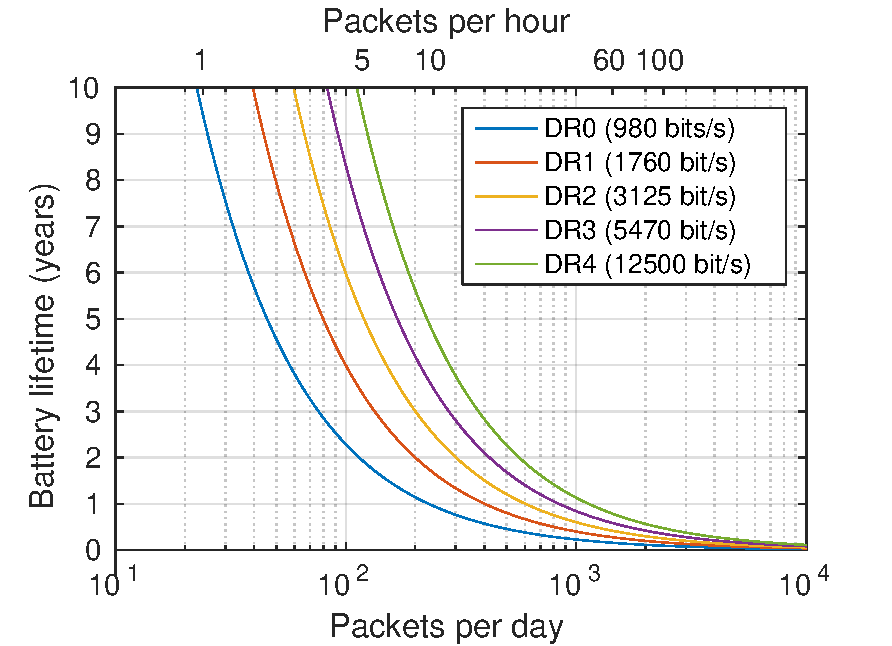
\includegraphics[width=0.36\textwidth]{figures/LoRaBug_AA_lifetime_semilog}
\label{fig:lifetime-estimates}}
\end{tabular}
\vspace*{-0.1in}
\caption{Power statistics}
\compactimg
\end{figure}

\section{Results}
\label{sec:eval}

%{\color{blue} }
%We implemented our system using 8 LPWAN boards as base stations distributed across a university campus.  We used a Semtech SX1276 LoRaWAN transmitter as the client device. We use Charm as the software platform at the backend to support backhaul. 

We evaluate Charm both through
proof-of-concept experiments and large-scale trace-driven simulations. We
perform our experiments in various environments (indoors and outdoors) across the campus. 




\subsection{Role of Transmission Rates on Battery Life}
\label{sec:energy-savings}


% Most LP-WAN client devices are expected to be small, low-cost and low-maintenance battery-operated devices performing primarily some sensing functions. As these devices are expected to operate for many years, battery life is a major concern and is very difficult to optimize for. The amount of data to transmit is determined by the device and we do not attempt to alter it in this paper. Similarly, to maintain compatibility, we do not alter the MAC protocols or client device requirements specified in LoRaWAN.

We study the energy profile of a typical battery-operated LoRaWAN client, as in \figref{power-trace}. The device performs some local computation, sends a LoRa message, waits for an acknowledgement and then goes to low-power sleep mode. The radio transmission consumes the highest amount of energy ($= \text{area under the curve} \times \text{voltage}$) by a large margin. Thus, any optimization to battery life must focus on reducing the energy of transmissions.

Two parameters affect the energy consumed by transmissions: (1) transmit power and (2) transmit time. Using the currently available LoRa radio chipsets (Semtech SX1272 and SX1276), we've observed that the transmit power does not significantly change the power drawn from the battery during transmission. Any optimization will thus have to focus on reducing the transmit time. The transmit time is determined by the data rate and the amount of data to send. We do not control the amount of data generated by client devices and thus, improving the data rate would provide the largest improvements.

\begin{figure}[!h]
\centering
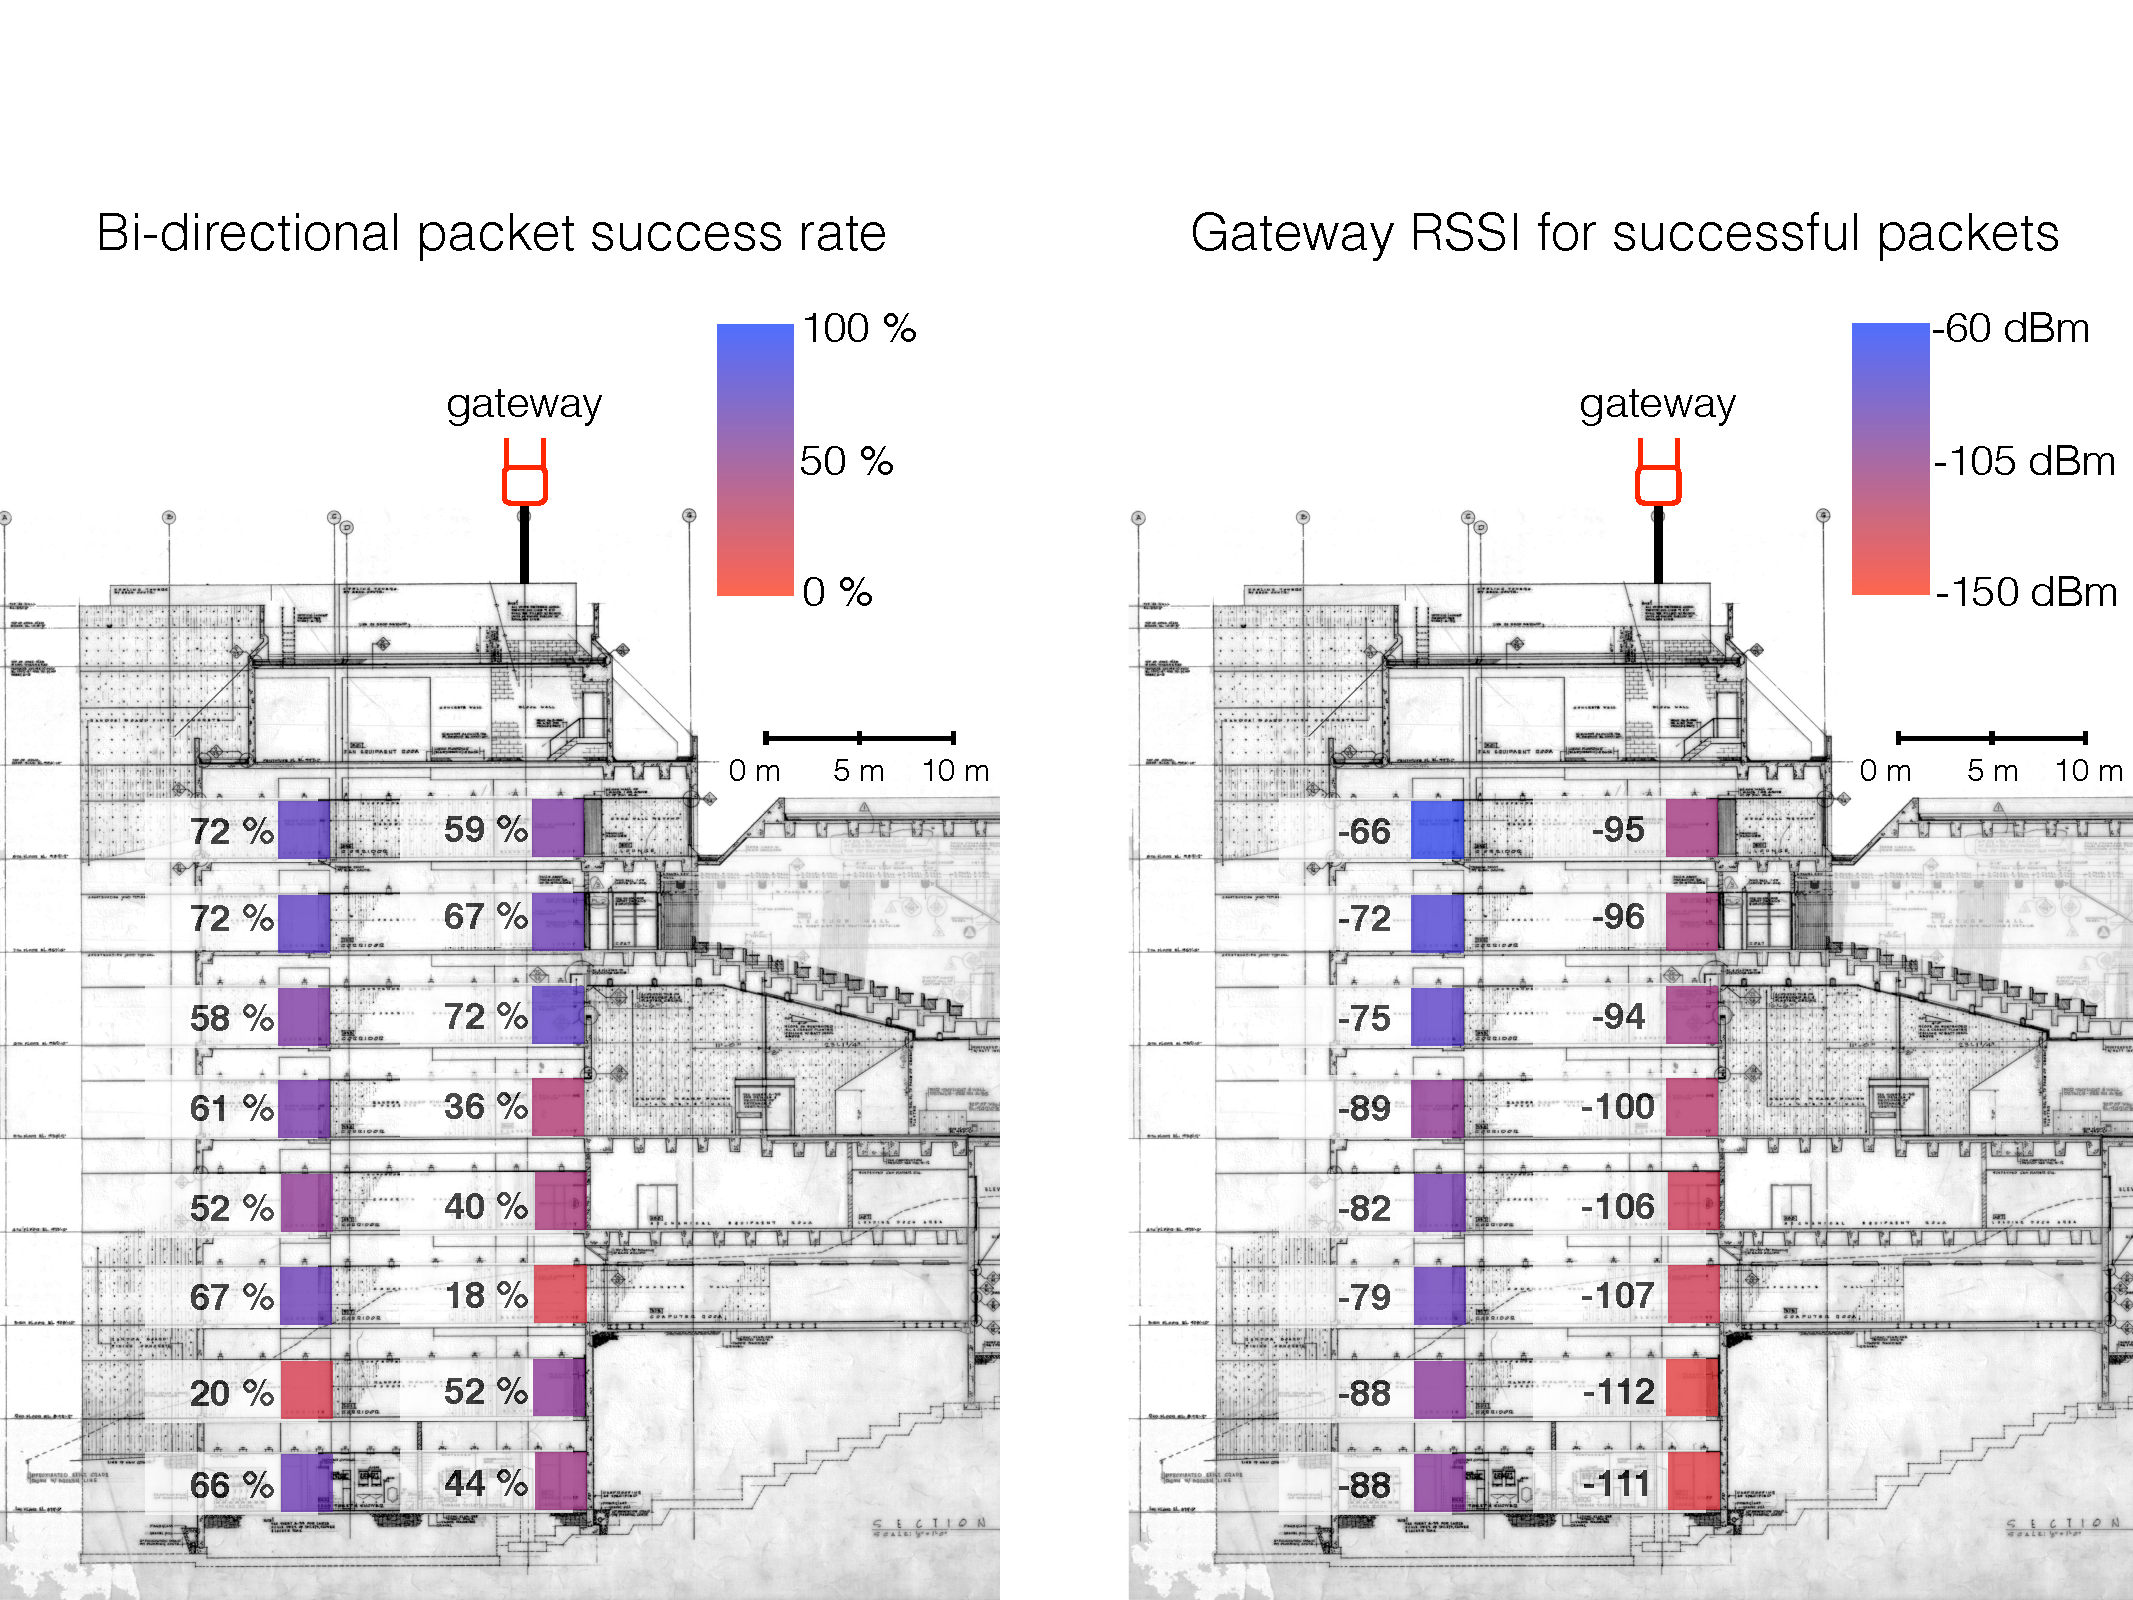
\includegraphics[width=0.35\textwidth]{figures/penetration_test_wean_cropped}
\caption{RF signal penetration experiments in a large poured-concrete building. (Left): the success rate for bi-directional packet exchange between end-node and gateway. (right): the RSSI at the gateway for successful transfers.}
\label{fig:penetration-test}
\compactimg
\end{figure}

\figref{lifetime-estimates} shows the estimated battery life of a client device if it were to communicate with different data rates. Wireless systems try to communicate at the highest data rate that does not cause too many errors. In the case of LoRa devices, switching to a slower data rate increases the spreading factor,  which have better sensitivity on the receiver. Thus, LoRa devices communicating at the highest spreading factors (and correspondingly using the lowest data rates) can communicate at much longer range and with higher reliability. The doenside is a significant increase in their transmission time which severely affects battery life. This demonstrates that Charm can significantly improve battery life should it allow clients to transmit at higher data rates. 

\begin{figure*}
\hfill
\begin{minipage}{.32\textwidth}
\centering
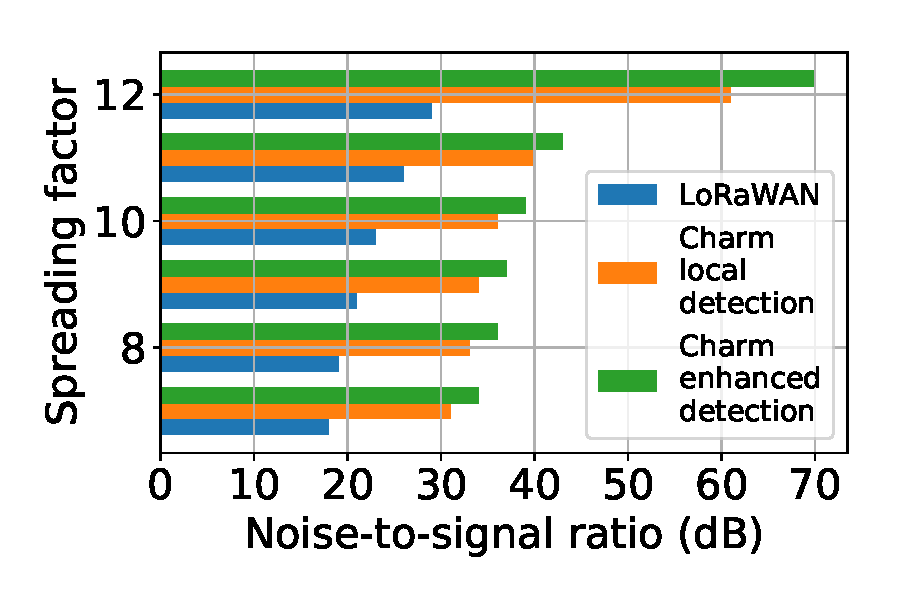
\includegraphics[width=0.95\textwidth]{figures/local_detection_limits}
\hspace*{-0.1in}
\caption{Local detection capacity at gateway for low SNRs}
\label{fig:local-detection}
\compactimg
\end{minipage}
\hfill
\begin{minipage}{.32\textwidth}
\centering
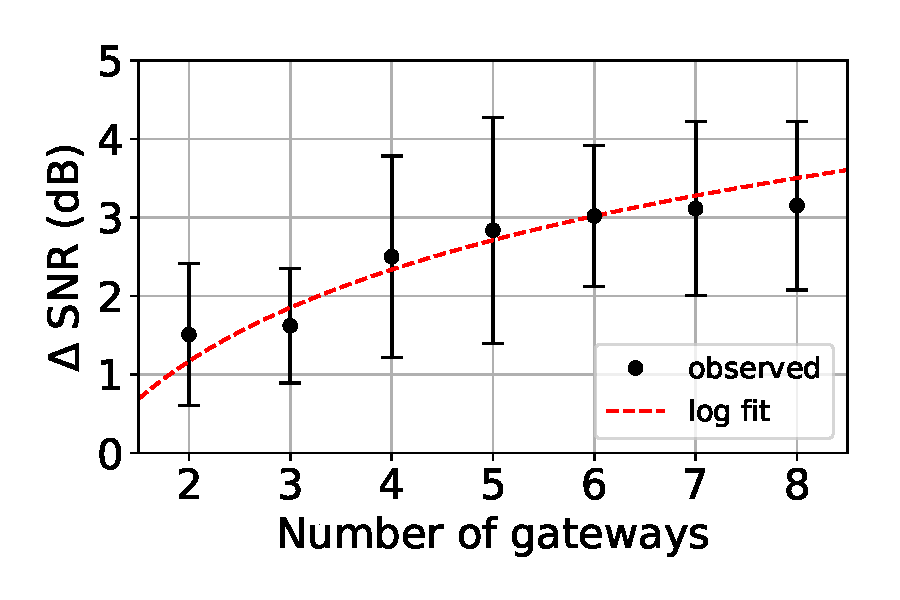
\includegraphics[width=0.95\textwidth]{figures/diversity_gain}
\hspace*{-0.1in}
\caption{Diversity gain with number of base stations}
\label{fig:diversity-gain}
\compactimg
\end{minipage}
\hfill
\begin{minipage}{.32\textwidth}
\centering
% Placeholder for adwait: Battery drain graph
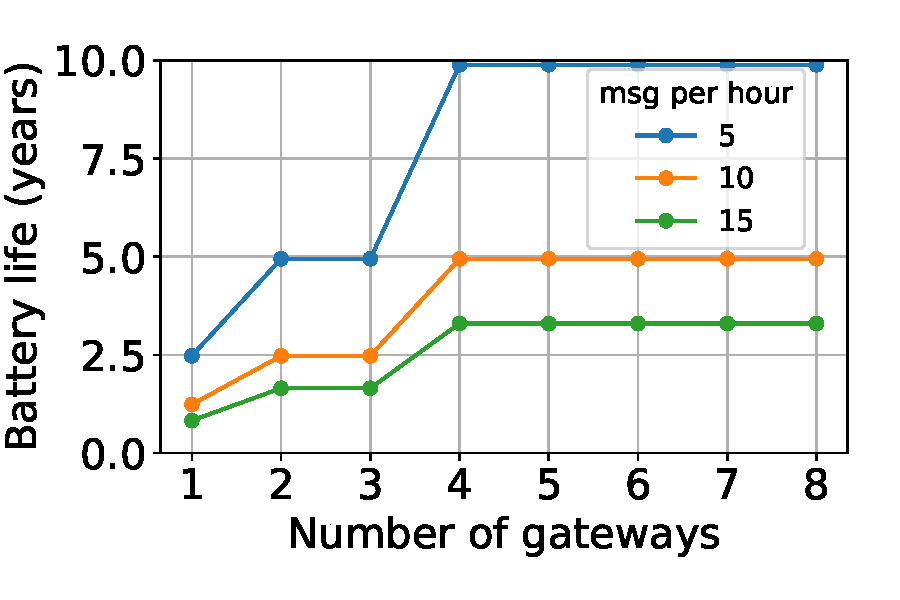
\includegraphics[width=0.95\textwidth]{figures/diversity_battery}
\hspace*{-0.1in}
\caption{Increase in battery life with number of base stations}
\label{fig:diversity-battery}
\compactimg
\end{minipage}
\end{figure*}

% Using Charm's joint decoding strategy, we enable devices previously forced to use low data rates due to distance or bad coverage, to communicate at higher data rates and lengthen their battery life. Devices which could previously communicate with at least one base stations using the highest data rate reliably, thus gain no benefit from Charm.



Charm can not only increase range but also increase coverage in urban scenarios with lots of obstructions and devices deep inside buildings. \figref{penetration-test} shows a penetration test experiment inside an on-campus poured-concrete building. Despite a gateway being placed on the roof of the building, we observe the received signal strength to vary as much as 46 dBm at various locations inside the building. A number of client devices, deep inside structure, would have been forced to use the the slowest data rate but can now benefit from Charm.

\subsection{Local detection algorithm}
\label{sec:local-detection-eval}


We performed trace-driven simulation to demonstrate the increase in detection capability of LoRa packets under noise. To perform this experiment, we collect data at different spreading factors at high SNRs. We then measure the signal power and progressively increase additive white Gaussian noise in the signal. At every dB of decrease in SNR, we test the state-of-the-art LoRaWAN decoding algorithm against Charm's local and enhanced detection algorithm, where the former uses the preamble alone and the latter uses both preamble and data in its optimization. 

The results in \figref{local-detection} show that Charm's local detection algorithm far outperforms the LoRaWAN detection algorithm for detection of the packet. Further, Charm's enhanced algorithm outperforms Charm's local detection algorithm by up to 10 dB, as it uses data symbols in addition to the preamble, improving performance. This demonstrates the value of using data symbols to better optimize packet detection, particularly in noisy settings. Our results also reveal a 33\% increase in the negative SNR under which a packet can be detected, when compared to LoRaWAN -- a gain of between 16-30 dB. To put this in perspective, this is equivalent boost in SNR by coherent combining of between 40-1000 gateways. Said differently, Charm can even detect packets that can only be decoded by coherently combining signals from at least 40 gateways that receive the same signal at a similar level of noise. 

% Swarun: Doesn't flow well
%Our results also reveal a 33\% increase in the negative SNR under which a packet can be detected, when compared to LoRaWAN. This increase of 33\% in power directly results in increase in coverage area of LoRa and improvement in battery-life for users already within coverage area. We also highlight how the enhanced algorithm is able to leverage the nature of the data to increase the quality of detection at extremely low SNRs. This shows that this algorithm can detect packets even under heavy noise from far or occluded locations which allows us to only send data to the cloud only when we detect the arrival of a packet. This lowers the bandwidth usage of the backbone network by reducing the amount of data that needs to be sent to the cloud. 
\subsection{Diversity gain}
\label{sec:diversity-gain-eval}

\cmt{}{Describe test testbed setup}

Next, we evaluate the  gain introduced by Charm in SNR when coherently combining the multiple transmissions from geographically diverse receivers at a central server.  \akshay{We perform these micro-benchmarks using eight indoor user-deployed gateways built using our custom hardware platform on a testbed covering an area of 0.6 km$^2$. Note that this testbed spans multiple buildings and open spaces between them and is supposed to emulate a dense urban deployment.}  We measure the mean and standard deviation in SNR improvement as a function of number of gateways across experiments.  

Our results reveal remarkable SNR improvements, which as expected improves steadily with an increasing number of gateways as depicted in Figure \ref{fig:diversity-gain}, for clients in different locations across multiple spreading factors. We note that the SNR gain improvement is logarithmic given that it is measured in dB (a log-scale). Across experiments, Charm gave an average observable improvement of 1 dB with the addition of each new receiver. This improvement is valuable, given that every 3 dB of gain allows us to use the next spreading factor. Any increase in spreading factor halves the transmission air time and the resulting energy expenditure. \figref{diversity-battery} depicts the improvement in battery life of an indoor LoRaWAN client with an increasing number of gateways collaborating to decode its signal. We observe that the battery life for a device transmitting 5 messages per hour at SF11 improves from 2.5 years to 10 years (SF9) with 4 or more collaborating gateways


\subsection{Range Improvement for Indoor User-Deployed Gateways}
\label{sec:indoor-udgs}
In typical urban settings, users will deploy large number of LoRa gateways. This increase in number of gateways reduces the range of a LoRa device and the bit-rate it can support even for hundreds of meters. \akshay{We deploy Charm in a highly congested urban building and demonstrate that collaboration improves the maximum range the LoRa device can support at any given data rate.}


\begin{wraptable}{r}{4.5cm}
%\vspace*{-0.1in}
\centering \begin{tabular}{||c | c | c||} 
 \hline
  & \textbf{SF7} & \textbf{SF10} \\ [0.5ex] 
 \hline\hline
 \textbf{LoRa} & $<$60m & $<$60m  \\ 
 \hline
 \textbf{4 UDGs} & $<$60m & $<$100m  \\
 \hline
 \textbf{8 UDGs} & $<$200m & $<$200m \\
 \hline
\end{tabular}
\caption{Range in congested indoor urban settings}
\label{tab:range}
\vspace*{-0.1in}
\end{wraptable}

Our results are shown in Table~\ref{tab:range}. \akshay{We compare the results of the LoRa gateway which is nearest to the transmitter with those of Charm with 4 and 8 gateways collaborating, respectively. Note that the ranges we observe here are smaller than outdoor gateways, owing to attenuation inside buildings and limited transmission power.}
\cmt{We compare the results of
a single LoRa gateway with those of Charm with 4 and 8 gateways collaborating,
respectively. Note that the ranges we observe here are smaller than outdoor
gateways, owing to attenuation inside buildings and limited transmission
power.}{describe this properly... mention using distance to nearest gateway.}
In this context, native LoRaWAN can at best reach 60~m of maximum range from
any gateway. In contrast, Charm consistently supports higher maximum range at
each spreading factor. The results with Charm using eight collaborating
gateways show a marked improvement in range of 200 m, higher than 4
collaborating gateways at 100 m.



\begin{figure*}[htb]
\centering
\subfloat[Dense cells]{
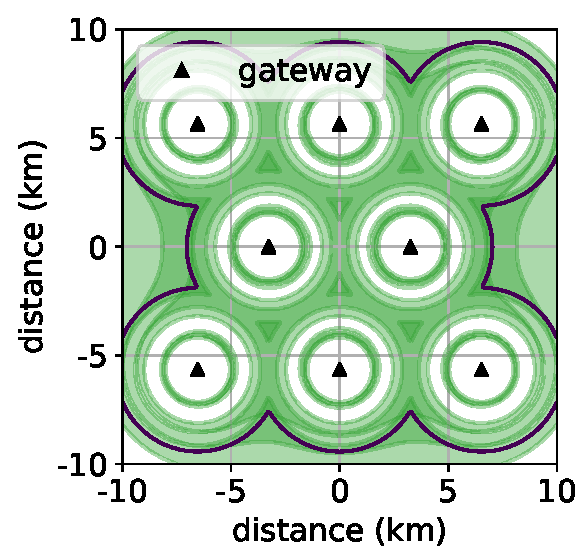
\includegraphics[width=0.3\textwidth]{figures/dense_cells_charm_improvement_cropped}
\label{fig:dense-improvement}
} \hfill
\subfloat[Sparse cells]{
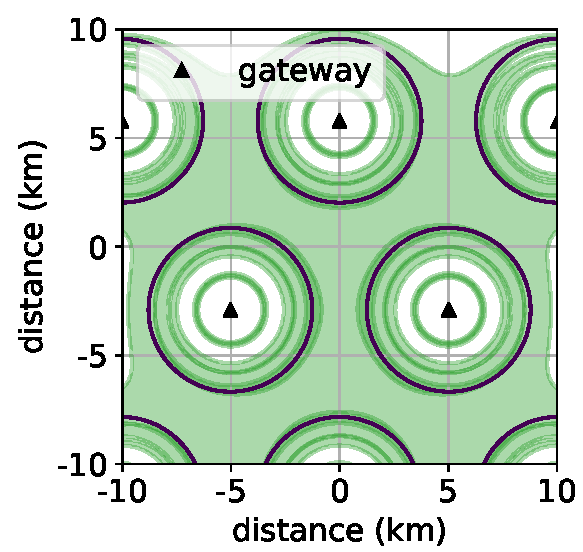
\includegraphics[width=0.3\textwidth]{figures/sparse_cells_charm_improvement_cropped}
\label{fig:sparse-improvement}
} \hfill
\subfloat[Random placement]{
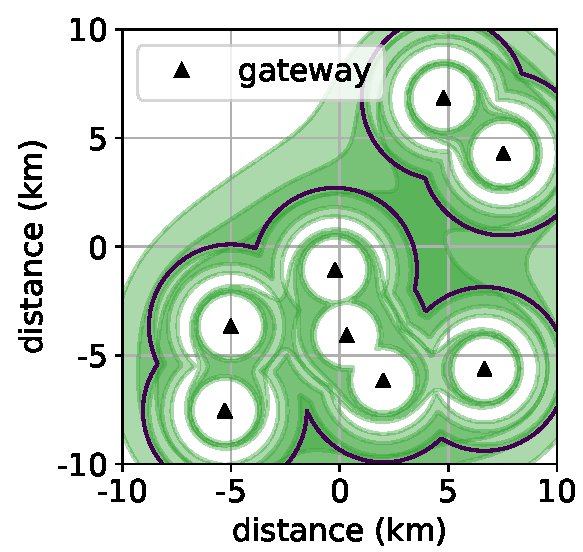
\includegraphics[width=0.3\textwidth]{figures/random_placement_charm_improvement_cropped}
\label{fig:random-improvement}
}
\compactimg
\caption{Improvement in coverage area and data rates due to Charm are shown by the green regions. The black lines show the coverage area with existing LoRaWAN. Darker regions denote greater gain in battery life.}
\label{fig:charm-improvement}
\compactimg
\end{figure*}


\subsection{Effect on coverage and client data rates}
\label{sec:coverage-data-rate-improvement}

This section uses trace-driven simulations to show the advantages of Charm in improving coverage area and client energy consumption in both planned and unplanned gateway deployments. We use the log-distance path loss model to estimate the signal power at any given receiver. The model is calibrated using 4850 points collected in a varied urban environment at varying data rates and spreading factors using a GPS-connected LoRa client device. Our log-distance parameters are $L_0  = 98.0729 dB$ for $d_0 = 40.0 m$, $\gamma = 2.1495$ and flat fading $\sigma^2 = 100.0724$. Sensitivity values for the gateway are taken from \cite{Bor2016} to determine the SNR threshold required to decode a transmission. Since this is an urban environment with many obstacles and reflectors, we observe a maximum range of 3.77 km using a transmit power of 15 dBm as opposed to the marketed range of 10 km with line-of-sight. We provide an optimistic estimate and ignore the effects of fading (assume $\sigma^2 = 0$) in the simulation, since we are interested in the trend of changes.

Assuming the same transmit power on the client of 15 dBm, \figref{charm-improvement} shows the region where Charm's local detection followed by joint decoding shows an improvement in either coverage, client data rates or both compared to independent decoding on gateways (as is currently done in LoRaWAN). Imagine the regions with no coverage having a data rate of DR``-1'' = 0 bps (the next lowest data rate is DR0 = 960 bps using SF = 12). Every shade of green represents a region where a client device can increase its data rate by one and correspondingly reduce its transmission time by approximately half. Darker green areas represent regions where devices can switch by more than one data rate. The areas enclosed within the black boundary are regions that could be covered by the existing LoRaWAN system (that decodes on each gateway independently). As can be seen in each of the sub-figures, Charm shows an improvement in the coverage area (green regions outside the existing coverage region), an increase in client data rates (green regions inside the existing coverage region) as well as both simultaneously (darker green areas outside the existing coverage area). Table~\ref{table:charm-improvements} shows the results of the simulations shown in \figref{charm-improvement}. Every increase in the data rate, doubles the battery life of a client device. Some regions in the simulation show up to 8 $\times$ energy savings.

\figref{dense-improvement} shows an ideal planned deployment where gateways are placed in a dense hexagonal grid 6.53 km apart from each other (corresponding to $2*3.77*\cos(\pi/6)$ km). Such an arrangement, popular in cellular deployments, provides optimal coverage with no gaps when using an independent decoding scheme. However, the points farthest from the gateways (e.g. on the centroid between three neighbouring gateways) have to use the slowest data rates (corresponding to SF12) and their battery life correspondingly suffers. If such a deployment were to be augmented with Charm, the region between the gateways can all communicate using SF9 or better. For the centroid points, this reduces the transmit time by approximately a factor of 8 and leads to huge energy savings. Additionally, we see the coverage area for joint decoding has expanded beyond the original coverage region. Some of the devices in the expanded coverage area can even communicate with higher data rates. An interesting phenomenon seen in each of the sub-figures are the thin concentric circles of improvement around each gateway. These are regions just outside the original boundaries covered by any given spreading factor that also gain a data rate increase due to joint decoding. However, this effect is not as prominent and the circles are small.

\figref{sparse-improvement} shows a sparse cellular arrangement with gateways 10.05 km apart from each other that can provide gap-free coverage. Charm thus enables decreasing the gateway density by a factor of 3.33 (proportional to square of inter-gateway distance $=(11.92/6.53)^2$) while providing the same level of coverage. Finally, we show in \figref{random-improvement} how Charm also improves the performance of an unplanned deployment of user-deployed gateways by improving coverage area as well as data rates for clients. Another interesting phenomenon to observe here is that Charm's joint decoding manages to fill in islands and orphaned regions. This is particularly relevant to urban regions where areas of bad coverage are formed in building basements and other indoor regions as seen in \figref{penetration-test}. 

\begin{table}[]
\centering
\caption{Summary of trace-driven simulation results shown in \figref{charm-improvement}}
\label{table:charm-improvements}
\begin{tabular}{l|l|l|l|}
\cline{2-4}
                                                       & \textbf{\begin{tabular}[c]{@{}l@{}}dense \\ cells\end{tabular}} & \textbf{\begin{tabular}[c]{@{}l@{}}sparse \\ cells\end{tabular}} & \textbf{\begin{tabular}[c]{@{}l@{}}random \\ placement\end{tabular}} \\ \hline
\multicolumn{1}{|l|}{\textbf{increase in coverage}}    & 46.60\%                                                         & 97.85\%                                                          & 74.59\%                                                              \\ \hline
\multicolumn{1}{|l|}{\textbf{data rate +1 (energy/2)}} & 35.33\%                                                         & 38.82\%                                                          & 33.70\%                                                              \\ \hline
\multicolumn{1}{|l|}{\textbf{data rate +2 (energy/4)}} & 22.30\%                                                         & 0\%                                                              & 25.82\%                                                              \\ \hline
\multicolumn{1}{|l|}{\textbf{data rate +3 (energy/8)}} & 2.26\%                                                          & 0\%                                                              & 3.48\%                                                               \\ \hline
\end{tabular}
\end{table}

\section{Conclusion and Future Work}
\label{sec:conclusion}

This paper presents Charm, a novel system that improves battery life and range
in LP-WANs clients. Charm achieves this through a mechanism that pools
together weak received signals across multiple gateways at the cloud in order
to jointly decode them. In doing so, Charm overcomes multiple challenges,
including a hardware-software design to detect weak signals at the gateway,
and ensure scalability at the cloud. A pilot evaluation of Charm on a network
of twelve LoRaWAN gateways serving a large neighborhood of a major U.S. city
demonstrates a large improvement in coverage and client battery-life.

An interesting side-benefit of Charm is its impact on scalability of the
network overall. Given that Charm improves coverage, one might expect a large
number of collisions from transmitters who newly gain coverage with existing
ones. Counter-intuitively, this is not the case because Charm allows devices
across the board to transmit at faster data rates, increasing available air
time in the network. Our future work will explore further improving network
scalability along two dimensions: (1) First, a full-scale distributed MIMO
system atop LP-WAN in the cloud, that can also handle collisions from a large
number of clients. (2) Second, offloading of TV whitespace spectrum at peak
demand, based on an FCC license recently granted to our university.



% This paper presents a novel location-aware network management system for
% LoRa-class LP-WANs operating in unlicensed and whitespace frequencies. It
% presents an RF-based localization system that stitches together information
% across frequencies to improve positioning accuracy of LoRa clients, even
% without access to their channel state information. We build on the
% localization framework to build a resource allocation system for LP-WAN that
% efficiently allocates wireless resources subject to FCC's regulatory
% constraints.  Our network-management system  is designed to be
% location-aware, exploiting live measurements to identify and respond to
% interference and help network managers plan changes to deployment. Our
% system was implemented and deployed in a large university campus and results
% from proof-of-concept experiments and large-scale trace-driven simulations
% are presented. In the future, we aim to expand our deployment to incorporate
% transmissions on the white spaces and are currently engaged in efforts to
% procure the relevant licenses. We also intend to integrate smart sensor
% devices currently deployed on-campus with LoRaWAN radios to evaluate our
% network management platform live and at-scale.

\section*{Acknowledgment}

This research is supported in part by the National Science Foundation under
award CNS-1329644 and the CONIX Research Center, one of six centers in JUMP, a
Semiconductor Research Corporation (SRC) program sponsored by DARPA.

\bibliographystyle{ACM-Reference-Format}
\bibliography{references} 

\end{document}
